\documentclass{revision_assets/ieeeaccess_revision}
\usepackage[T1]{fontenc}
\usepackage{mathptmx}
\usepackage{cite}
\usepackage{amsmath,amssymb}
\DeclareMathOperator*{\argmax}{arg\,max}
\usepackage{algorithmic}
\usepackage{graphicx, multirow, adjustbox, float}
\usepackage[table]{xcolor}
\usepackage{soul}
\usepackage{framed}
\newif\ifrevisionhighlights
\revisionhighlightsfalse
\definecolor{shadecolor}{RGB}{255,255,160}
\newenvironment{revision}{\ifrevisionhighlights\begin{shaded*}\fi}{\ifrevisionhighlights\end{shaded*}\fi}
\newcommand{\pending}[1]{\textcolor{red!70!black}{\textbf{Pending evidence:} #1}}
\sethlcolor{yellow}
\usepackage{caption, subcaption}
\usepackage{siunitx}
\sisetup{ group-separator = {,}, group-minimum-digits = 4}
\usepackage{hyperref}
\usepackage{booktabs}
\usepackage{subcaption}

\def\BibTeX{{\rm B\kern-.05em{\sc i\kern-.025em b}\kern-.08em
T\kern-.1667em\lower.7ex\hbox{E}\kern-.125emX}}

\begin{document}
\history{Working revision draft; experimental evidence pending.}
\doi{}
\title{FKANMamba: FastKAN-Enhanced State Space Learning for Spectral-Spatial Hyperspectral Image Classification}
\author{\uppercase{Muhammad Arslan}\authorrefmark{1},
\uppercase{Jae Hyeon Kim\authorrefmark{1}, Muhammad Hassaan Farooq Butt}\authorrefmark{2}, and Jay Hoon Jung\authorrefmark{1}}
\address[1]{Department of Computer Engineering, Korea Aerospace University, Gyeonggi-do 10540,  Republic of Korea (e-mail: arslan@kau.ac.kr)}
\address[2]{Faculty of Environmental Sciences and Natural Resource Management (MINA), Norwegian University of Life Sciences (NMBU), 1432 Ås, Norway (e-mail: mubut0522@nmbu.no)}

\corresp{Corresponding author: Jay Hoon Jung (e-mail: jhjung@kau.ac.kr).}

\begin{abstract}
\begin{revision}
We investigate FKANMamba, a patch-based hyperspectral classifier combining radial-basis-function FastKAN mappings, two-branch attention, and a non-selective affine recurrent state-space aggregator. Independent token projections and context-derived channel gates precede shared nonlinear attention. The model identifier does not imply an implementation of selective Mamba. Historical experiments on five hyperspectral scenes report high within-scene classification accuracy and a compact parameter count relative to the listed Transformer and KAN baselines. Those results use overlapping random-pixel neighborhoods and full-scene PCA; they do not establish spatially independent generalization, repeated-run reliability, or comparative runtime superiority. The revision specifies controlled projection and aggregation ablations, five independently seeded pipeline repetitions, and support-disjoint evaluation on HC and HH. \pending{The new experimental and computational results must be inserted before submission.}
\end{revision}
\end{abstract}
\begin{keywords}
Hyperspectral image classification (HSIC), Fast Kolmogorov-Arnold Network (KAN), State-space models (SSMs), Spectral-Spatial feature learning
\end{keywords}

\titlepgskip=-15pt
\maketitle

\section{Introduction}
\label{intro}
HSI captures reflectance across hundreds of narrow, contiguous wavelength bands, giving each pixel a spectral signature for the detailed discrimination of materials and land-cover categories \cite{ref1}. This spectral richness has been used in Earth observation, mineral exploration, environmental monitoring, climate-related studies, and other domain-specific analysis tasks \cite{ref2,ref4,ref5,ref6,ref7,ref8,ref9,ref_itt}. Despite these advantages, HSIC remains challenging because high spectral dimensionality introduces substantial redundancy, whereas labeled samples are often limited \cite{ref_act}. Classification is further complicated by spectral similarity among classes, within-class spectral variability, and heterogeneous local neighborhoods in which boundary pixels may exhibit mixed responses from multiple materials.

Among deep learning approaches, Convolutional neural networks (CNNs) are widely used to directly extract local spectral-spatial features from HSI patches \cite{ref10,ref11,ref12,ref13,ref14}. In particular, 3D convolutions can jointly model inter-band correlations and local spatial structures within spectral-spatial cubes. However, convolutional feature aggregation is mainly governed by local receptive fields, which may limit the modeling of dependencies between distant spatial or spectral positions. This constraint can affect the discrimination of spectrally similar classes and increase sensitivity to heterogeneous spatial neighborhoods \cite{ref15,ref16}.

To overcome the locality limitation of CNNs, ViT-based HSIC methods represent HSI patches as sequences of tokens. These methods use self-attention mechanisms to capture dependencies that extend beyond local convolutional regions \cite{ref17,ref18,ref19}. Although self-attention enables global token interactions, its computational cost scales quadratically with sequence length. Moreover, conventional attention usually constructs query, key, and value representations through linear projections. Such linear transformations may be insufficient to fully characterize subtle nonlinear differences among classes with overlapping spectral signatures.

SSMs, including Mamba-based architectures, have recently provided an efficient alternative for sequence modeling with linear complexity in the sequence length \cite{ref20,ref21}. SSM-based HSIC methods have introduced spectral smoothing, multidimensional sequence construction, and graph-guided spatial aggregation to improve spectral-spatial context modeling \cite{ref22,ref23,ref_dima}. However, state-space propagation operates on the token representations supplied to the sequence model. It does not explicitly refine noisy feature responses or enhance nonlinear discriminative transformations before sequential processing. Therefore, the classification performance of an SSM-based HSIC model remains strongly dependent on the quality of its input token sequence.

Furthermore, KANs replace fixed linear transformations with learnable basis-function mappings. In HSIC, existing KAN-based methods have applied these mappings for feature extraction and as a replacement for conventional linear, convolutional, and feed-forward operators. Taylor-series and frequency-aware formulations have also been explored to reduce computational costs or modify the nonlinear basis representation. Some studies \cite{ref24,ref25,ref26,ref27,ref28} have shown the potential of KAN-based nonlinear transformations for HSIC. However, the coordinated use of KANs for feature conditioning before token interaction, nonlinear query-key-value construction during attention, and subsequent state-space propagation has received less attention. This coordination is important for HSI patches because noisy neighborhood responses may directly enter attention, whereas linearly projected tokens may not adequately represent subtle class-dependent spectral variations.

To overcome this limitation, we propose FKANMamba, a spectral-spatial HSIC architecture that integrates radial basis function (RBF)-based FastKAN transformations with attention and state-space sequence modeling. Independent learnable projections first generate complementary spectral and spatial token representations from an HSI patch. A FEB then performs nonlinear channel-wise modulation to refine these representations before attention. The FSSA module further replaces conventional linear query, key, and value projections with RBF-based FastKAN mappings to model nonlinear token dependencies. Finally, the resulting attention features are fused and processed by a state-space sequence module to aggregate context before classification.

\begin{revision}
The contribution is an investigated combination of established operators: RBF-based channel gating and query/key/value mappings are integrated with two token views and an affine recurrent aggregator. We provide an explicit account of the implemented tensor operations and qualify the evidence to within-scene classification. Controlled comparisons are required to establish whether the RBF mappings and recurrent readout improve on simpler alternatives; their individual superiority is not established by the historical complete-model results.
\end{revision}

\begin{figure*}[!t]
    \centering
    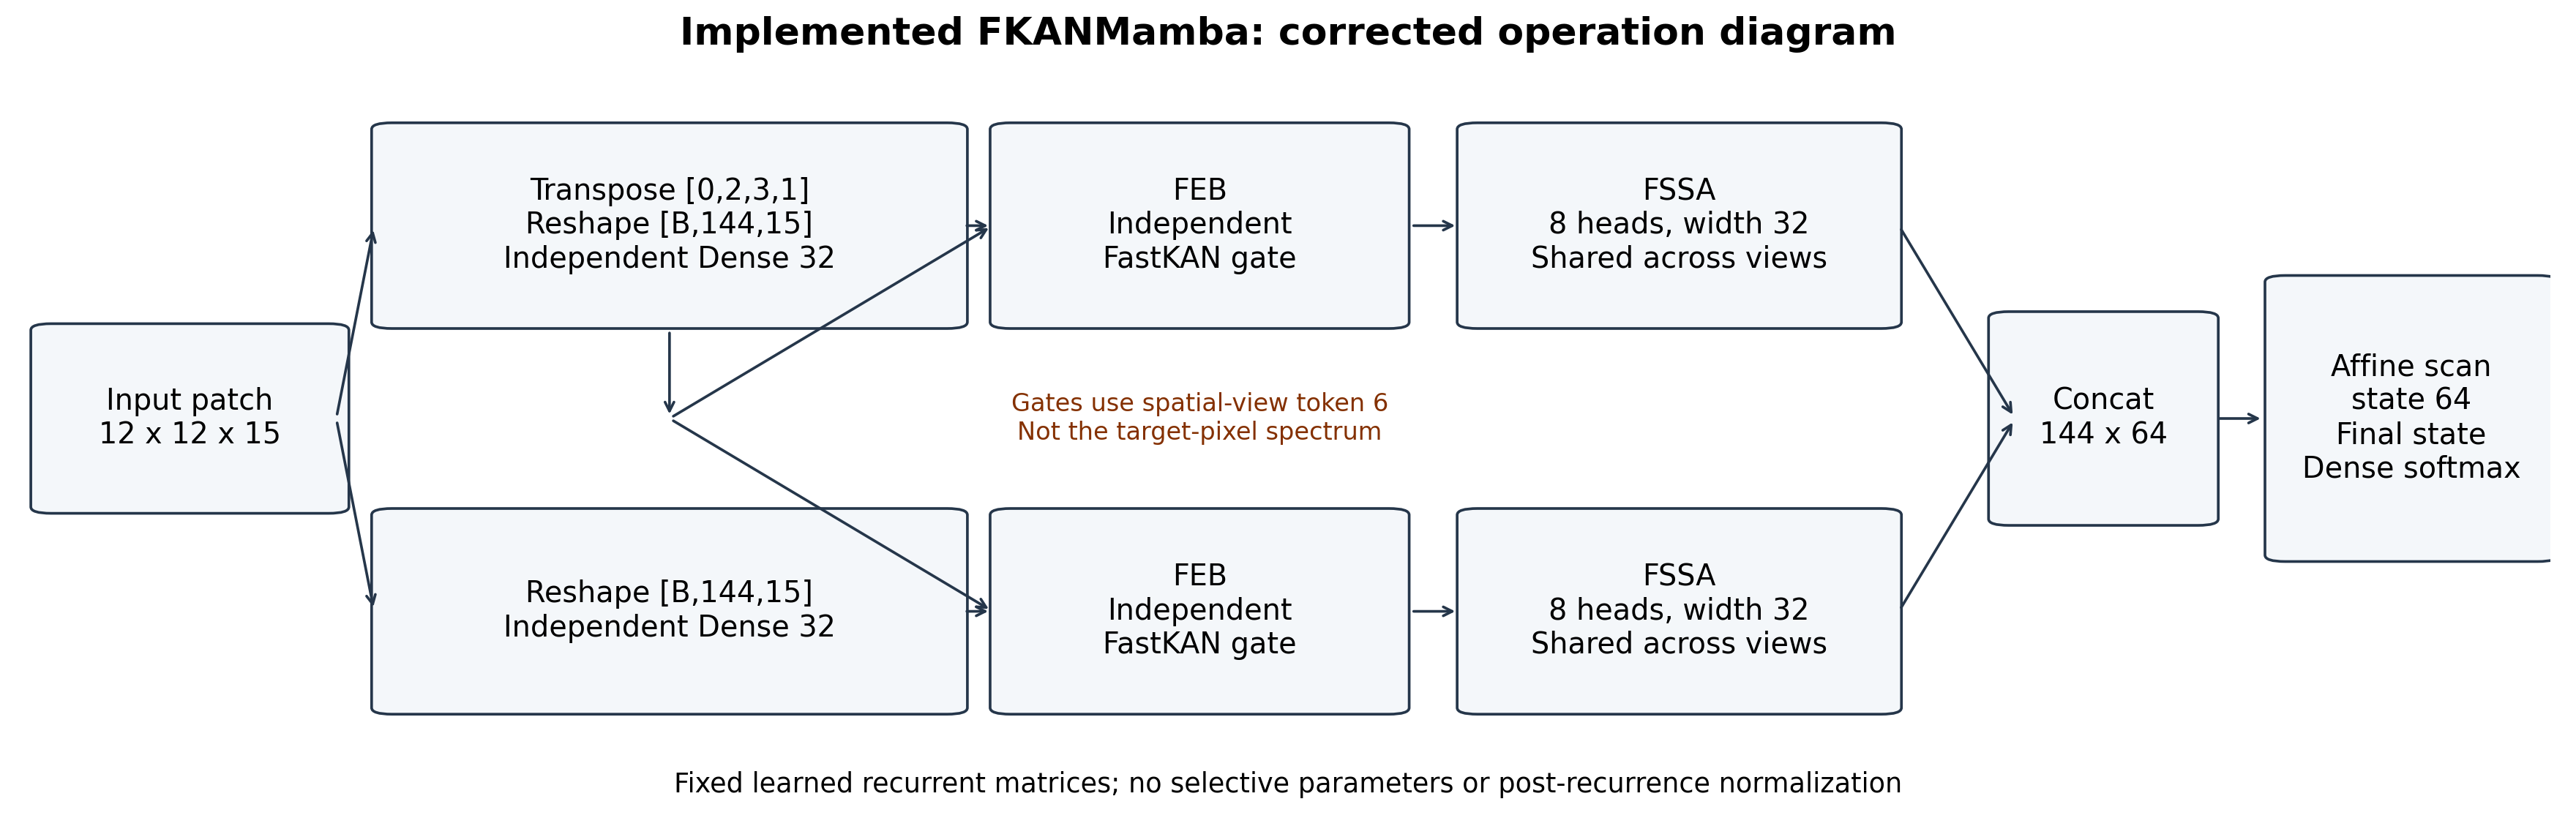
\includegraphics[width=\textwidth]{revision_assets/figures/architecture.png}
    \caption{Revised operation diagram. FKANMamba uses two tensor-order token views, independent projections and FEB gates, shared FastKAN attention, indexwise concatenation, and a non-selective affine recurrent aggregator. FEB uses a fixed representative token, not the target-pixel spectrum. A dense softmax classifier reads the final hidden state; no post-recurrence normalization is used.}
\label{fig:architecture}
\end{figure*}
\begin{revision}
\textbf{Working revision status.} Historical tables are retained as single-run within-scene observations. The five-repetition, spatial, controlled-ablation, and profiling studies described in Section~\ref{sec:revision_protocol} are specified but not yet completed. This manuscript is not submission-ready.
\end{revision}

\section{Proposed Methodology}

In the HSIC, each pixel is characterized by a spectral signature capturing reflectance across multiple wavelength bands. Let $\mathbf{X}\in\mathbb{R}^{H\times W\times C}$ denote an HSI cube, where $ H$ and $ W$ are the spatial dimensions and $C$ is the number of spectral bands. To reduce spectral redundancy and computational cost, the original spectral dimension is first reduced to $C_r$ components. For each labeled pixel, an overlapping patch $\mathbf{P}_{i,j}\in\mathbb{R}^{p\times p\times C_r}$ is extracted from the reduced HSI cube. Each patch is then converted into token sequences and processed by the proposed FKANMamba model.

FKANMamba consists of four main stages. First, two branch-specific token views are generated from the PCA-reduced HSI patch using different tensor orderings and independent learnable projections. Second, the FEB utilizes nonlinear, channel-wise modulation to enhance the spectral and spatial branch tokens before the attention mechanism. Third, the FSSA module replaces conventional linear query, key, and value projections with RBF-based FastKAN mappings. Finally, the fused attention features are passed to a lightweight recurrent state-space module for sequential context aggregation, followed by a classification layer. Figure~\ref {fig:architecture} describes the proposed architecture.

\subsection{Token Generation}
\label{sec:token_details}
\begin{revision}
Let $\mathbf X\in\mathbb R^{B\times p\times p\times C_r}$. The implementation constructs $L=p^2$ tokens per branch using
\begin{equation}
\begin{aligned}
F_{\rm spec}&=\operatorname{reshape}(X,[B,p^2,C_r]),\\
F_{\rm spa}&=\operatorname{reshape}(\operatorname{transpose}(X,[0,2,3,1]),[B,p^2,C_r]).
\end{aligned}
\label{eq:patch_tokens}
\end{equation}
These are different memory-order views, not two pixel-aligned sequences. With zero-based token index $t$ and feature index $j$, put $q=tC_r+j$. Then
\begin{equation}
\begin{aligned}
F_{\rm spec}[b,t,j]&=X[b,\lfloor t/p\rfloor,t\bmod p,j],\\
F_{\rm spa}[b,t,j]&=X[b,q\bmod p,\lfloor q/(C_rp)\rfloor,\lfloor q/p\rfloor\bmod C_r].
\end{aligned}
\end{equation}
The latter groups entries from multiple spatial rows and PCA components. Each sequence is projected through its own biased dense map from $C_r=15$ to $d=32$. The projections do not share weights. At fusion, equal sequence indices are concatenated along the channel axis; equal indices do not imply a common physical pixel. Thus the branches are complementary tensor views, and no pixelwise alignment claim is made.
\begin{equation}
S_{\rm spa}=F_{\rm spa}W_{\rm spa}+b_{\rm spa},\qquad
S_{\rm spec}=F_{\rm spec}W_{\rm spec}+b_{\rm spec}.
\label{eq:tokens}
\end{equation}
\end{revision}
\subsection{Fast Kolmogorov-Arnold Network}
\label{sec:fastkan}
\begin{revision}
All implemented FastKAN maps use eight Gaussian RBF centers initialized uniformly over $[-1,1]$, with fixed initial spacing $2/7$ in the denominator. The centers themselves are trainable; the initial interval is not a constraint on their subsequent values. Feature-axis LayerNorm precedes the basis expansion. The optional base-update branch is disabled. Spline projection weights use Glorot-uniform initialization and an L2 penalty of 0.001; the constructor's spline initialization-scale argument does not control the active initializer.
\end{revision}


KANs parameterize nonlinear transformations through learnable basis-function mappings. Standard KAN implementations commonly use B-spline bases, but spline evaluation and grid adaptation can increase computational costs. FastKAN \cite{ref29} provides a lighter alternative by using Gaussian RBF expansions. In FKANMamba, this FastKAN formulation is used for channel-gate generation in FEB and for nonlinear query, key, and value construction in FSSA.

Let $\mathbf{Z}\in\mathbb{R}^{B\times L\times d_{\mathrm{in}}}$ denote an input token sequence. The input representation is first normalized across the feature dimension:
\begin{equation}
\widetilde{\mathbf{Z}}
=
\operatorname{LN}(\mathbf{Z})
\in
\mathbb{R}^{B\times L\times d_{\mathrm{in}}}.
\label{eq:fastkan_norm}
\end{equation}
Each normalized feature value is expanded using $M$ Gaussian RBFs. Let
$\mathbf{g}=[g_1,g_2,\ldots,g_M]$ denote the grid centers, which are initialized uniformly over $[g_{\min},g_{\max}]$ and optimized during training. The grid spacing is defined as
\begin{equation}
h =
\frac{g_{\max}-g_{\min}}{M-1}.
\end{equation}
The response of the $m$-th basis function is computed by
\begin{equation}
\Phi_{b,l,j,m}
=
\exp
\left[
-
\left(
\frac{\widetilde{Z}_{b,l,j}-g_m}{h}
\right)^2
\right],
\label{eq:fastkan_rbf}
\end{equation}
where $b$, $l$, $j$, and $m$ index the batch, token position, feature channel, and RBF center, respectively. This produces
\begin{equation}
\boldsymbol{\Phi}
\in
\mathbb{R}^{B\times L\times d_{\mathrm{in}}\times M}.
\end{equation}
The feature and basis dimensions are flattened:
\begin{equation}
\boldsymbol{\Phi}_{\mathrm{flat}}
=
\operatorname{reshape}(\boldsymbol{\Phi})
\in
\mathbb{R}^{B\times L\times(d_{\mathrm{in}}M)}.
\end{equation}
The transformed output is then obtained through a learnable linear mapping:
\begin{equation}
\mathbf{Y}
=
\boldsymbol{\Phi}_{\mathrm{flat}}\mathbf{W}_{\mathrm{rbf}},
\qquad
\mathbf{W}_{\mathrm{rbf}}
\in
\mathbb{R}^{(d_{\mathrm{in}}M)\times d_{\mathrm{out}}},
\label{eq:fastkan_output}
\end{equation}
where $\mathbf{Y}\in\mathbb{R}^{B\times L\times d_{\mathrm{out}}}$. Thus, the FastKAN layer provides localized nonlinear feature responses via an RBF expansion, followed by a compact, learnable projection.

\subsection{FastKAN Enhancement Block}
\begin{revision}
FEB selects zero-based index $l_r=p/2=6$ from $S_{\rm spa}$ for the $12\times12$ setting. The target pixel lies at patch coordinate $(6,6)$ under offsets $-6,\ldots,+5$; its row-major pixel-token index would be 78. The selected transposed-branch token is not that pixel's spectrum. We therefore call it a fixed representative token. Independent FastKAN maps followed by sigmoid generate the two channel gates, which are broadcast over token positions. This description preserves the inspected local computation; identity with the historical run configuration requires verification.
\end{revision}

\label{sec:feb}

The FEB refines the spectral and spatial branch tokens through adaptive channel-wise modulation before attention. Let
$\mathbf{S}_{\mathrm{spa}},\mathbf{S}_{\mathrm{spec}}\in\mathbb{R}^{B\times L\times d}$ denote the token embeddings. FEB first selects a representative token from the spatial branch:
\begin{equation}
\mathbf{S}_{c}
=
\mathbf{S}_{\mathrm{spa}}[:,l_r,:]
\in
\mathbb{R}^{B\times d},
\label{eq:feb_anchor}
\end{equation}
where $l_r$ denotes the selected representative token index. This token is used as a compact contextual descriptor for generating channel gates.

Two independently parameterized FastKAN mappings followed by sigmoid activation generate branch-specific gates:
\begin{equation}
\begin{aligned}
\mathbf{G}_{\mathrm{spa}}
&=
\sigma\left(
\operatorname{FastKAN}_{\mathrm{spa}}(\mathbf{S}_{c})
\right)
\in
\mathbb{R}^{B\times d}, \\
\mathbf{G}_{\mathrm{spec}}
&=
\sigma\left(
\operatorname{FastKAN}_{\mathrm{spec}}(\mathbf{S}_{c})
\right)
\in
\mathbb{R}^{B\times d},
\end{aligned}
\label{eq:feb_gate}
\end{equation}
where $\sigma(\cdot)$ denotes the element-wise sigmoid function. The gates are broadcast along the token dimension and applied to the corresponding branch features:
\begin{equation}
\begin{aligned}
\widetilde{S}^{\mathrm{spa}}_{b,l,j}
&=
S^{\mathrm{spa}}_{b,l,j}
G^{\mathrm{spa}}_{b,j}, \\
\widetilde{S}^{\mathrm{spec}}_{b,l,j}
&=
S^{\mathrm{spec}}_{b,l,j}
G^{\mathrm{spec}}_{b,j}.
\end{aligned}
\label{eq:feb_output}
\end{equation}
The enhanced representations are denoted by
$\widetilde{\mathbf{S}}_{\mathrm{spa}},\widetilde{\mathbf{S}}_{\mathrm{spec}}\in\mathbb{R}^{B\times L\times d}$. Since the gates are channel-wise, the same modulation vector is shared across all token positions within each patch.

\subsection{FastKAN Spectral-Spatial Attention}
\begin{revision}
The same FSSA layer instance is applied to both branches, so its query, key, value, and output-projection weights are shared across branches. The Q, K, and V mappings are mutually distinct. Each produces 32 channels, divided into eight heads of width four; the biased output projection also produces 32 channels. Attention-weight dropout is 0.7 during training. Concatenation therefore gives a fused width of 64.
\end{revision}

\label{sec:fssa}

After feature enhancement, FSSA models token-level dependencies within each branch. Conventional multi-head self-attention constructs query, key, and value tensors through linear projections. In FSSA, these projections are replaced with RBF-based FastKAN mappings, enabling nonlinear feature transformations prior to attention computation.

For $r\in\{\mathrm{spa},\mathrm{spec}\}$, the enhanced branch representation
$\widetilde{\mathbf{S}}_{r}\in\mathbb{R}^{B\times L\times d}$ is mapped to query, key, and value tensors as:
\begin{equation}
\begin{aligned}
\mathbf{Q}^{(r)}
&=
\operatorname{FastKAN}_{q}
\left(
\widetilde{\mathbf{S}}_{r}
\right),\\
\mathbf{K}^{(r)}
&=
\operatorname{FastKAN}_{k}
\left(
\widetilde{\mathbf{S}}_{r}
\right),\\
\mathbf{V}^{(r)}
&=
\operatorname{FastKAN}_{v}
\left(
\widetilde{\mathbf{S}}_{r}
\right),
\end{aligned}
\label{eq:fssa_qkv}
\end{equation}
where $\mathbf{Q}^{(r)},\mathbf{K}^{(r)},\mathbf{V}^{(r)}\in\mathbb{R}^{B\times L\times d_{\mathrm{out}}}$. The FastKAN-based attention layer is applied to both branches, which keeps the module compact while producing branch-specific attention outputs from different inputs.The projected tensors are split into $h$ heads, with $d_h=d_{\mathrm{out}}/h$. The attention is computed as
\begin{equation}
\mathbf{A}^{(r)}_{m}
=
\operatorname{softmax}
\left(
\frac{
\mathbf{Q}^{(r)}_{m}
\left(
\mathbf{K}^{(r)}_{m}
\right)^{\top}
}
{\sqrt{d_h}}
\right),
\label{eq:fssa_attention}
\end{equation}
where softmax is applied along the token dimension. Dropout is applied to the attention weights during training, and the head output is
\begin{equation}
\mathbf{O}^{(r)}_{m}
=
\operatorname{Dropout}
\left(
\mathbf{A}^{(r)}_{m}
\right)
\mathbf{V}^{(r)}_{m}.
\label{eq:fssa_head_output}
\end{equation}
The representations from all attention heads are aggregated and mapped as:
\begin{equation}
\widehat{\mathbf{O}}^{(r)}
=
\operatorname{Concat}
\left(
\mathbf{O}^{(r)}_{1},
\ldots,
\mathbf{O}^{(r)}_{h}
\right)
\mathbf{W}_{o}
+
\mathbf{b}_{o}.
\label{eq:fssa_output_projection}
\end{equation}
Finally, the spectral and spatial branch outputs are fused through feature concatenation:
\begin{equation}
\mathbf{O}
=
\left[
\widehat{\mathbf{O}}^{(\mathrm{spa})}
\parallel
\widehat{\mathbf{O}}^{(\mathrm{spec})}
\right]
\in
\mathbb{R}^{B\times L\times 2d_{\mathrm{out}}}.
\label{eq:fssa_fusion}
\end{equation}
The fused representation combines the two branch-wise attention outputs and is passed to the recurrent state-space module.

\subsection{Non-Selective Affine Recurrent State-Space Aggregator}
\label{sec:ssm}
\begin{revision}
The submitted recurrent module is an affine linear recurrent network with hidden width $d_s=64$. It scans fused indices $t=0,\ldots,143$ in their constructed order, starts at zero, and uses the final hidden state for classification:
\begin{equation}
h_{t+1}=h_tW_{\rm trans}+O_tW_{\rm update}+b_{\rm trans}+b_{\rm update},\qquad h_0=0.
\label{eq:ssm_update}
\end{equation}
Both dense maps include biases. Their parameters are learned but shared over positions, with no recurrent activation, input-dependent selection, or Mamba-specific discretization. Consequently this is a non-selective affine state-space aggregator, not an implementation of selective Mamba. FKANMamba is retained as the framework identifier. The classifier is a biased dense softmax applied directly to $h_L$; the separately declared dense/dropout members are unused in the forward pass. No normalization is applied between this hidden state and the classifier.
\begin{equation}
\widehat y=\operatorname{softmax}(h_LW_{\rm cls}+b_{\rm cls}).
\label{eq:ssm_softmax}
\end{equation}
Training uses categorical cross-entropy plus the regularization losses attached to active spline weights. For fixed widths, the recurrent scan costs $O(L(d_s^2+d_fd_s))$. The two attention calls retain $O(L^2d)$ arithmetic and $O(HL^2)$ attention-score storage, where $H$ is the head count. The shared weights reduce stored parameters but do not remove the second attention call. RBF expansion additionally costs $O(LdM)$ basis operations and $O(LdMd_{\rm out})$ projection arithmetic per mapping. The complete model therefore does not have linear complexity in token length. Parameter count alone does not establish runtime or memory superiority.
\end{revision}

\section{Experimental Settings and Dataset Information}
\label{sec:experiments}

FKANMamba was evaluated on five publicly available HSI benchmarks: QUH-Pingan (PI), QUH-Qingyun (QUH), QUH-Tangdaowan (TH), WHU-Hi-HanChuan (HC), and WHU-Hi-HongHu (HH). Together, these datasets cover a range of acquisition environments, including coastal, urban, wetland, and agricultural regions, thereby providing diverse conditions for assessing spectral-spatial classification performance. Their principal characteristics are listed in Table~\ref{tab:hsi_datasets}. PI, QUH, and TH were collected in Qingdao, China, using a UAV-based Gaiasky mini2-VN HSI system~\cite{ref30}. PI represents a coastal scene containing marine, infrastructure, and land-cover categories, whereas QUH primarily contains urban surface and object classes. TH provides a more heterogeneous wetland environment composed of vegetation, exposed soil, and artificial structures.
\begin{table}[!hbt]
% \tiny
\centering
\caption{Summary of the HSI datasets}
\resizebox{\columnwidth}{!}{\begin{tabular}{|c|c|c|c|c|c|c|}
\hline
\textbf{Characteristic} & \textbf{TH} & \textbf{PI} & \textbf{QUH} & \textbf{HC} & \textbf{HH} \\
\hline
Sensor & Gaiasky mini2-VN & Gaiasky mini2-VN & Gaiasky mini2-VN & UAV & UAV \\
\hline
Wavelength (nm) & 400--1000 & 400--1000 & 400--1000 & 400--1000 & 400--1000 \\
\hline
Resolution (mpp) & 0.15 & 0.10 & 0.15 & 0.109 & 0.043 \\
\hline
Spatial size & $1740 \times 860$ & $1230 \times 1000$ & $880 \times 1360$ & $1217 \times 303$ & $940 \times 475$ \\
\hline
Spectral bands & 176 & 176 & 270 & 274 & 270 \\
\hline
Classes & 18 & 10 & 6 & 16 & 22 \\
\hline
Platform & UAV & UAV & UAV & UAV & UAV \\
\hline
\end{tabular}}
\label{tab:hsi_datasets}
\end{table}


% \begin{table*}[!htbp]
%     \centering
%     \caption{Summary of the HSI datasets used for experimental evaluation.}
%     \label{tab:hsi_datasets}
%     \setlength{\tabcolsep}{4pt}
%     \begin{tabular}{|c|c|c|c|c|c|c}\hline
%     \textbf{Characteristic} & \textbf{TH} & \textbf{PI} & \textbf{QUH} & \textbf{HC} & \textbf{HH} \\\hline
%     Sensor                  & Gaiasky mini2-VN & Gaiasky mini2-VN & Gaiasky mini2-VN & UAV & UAV \\
%     Wavelength (nm)         & 400--1000 & 400--1000 & 400--1000 & 400--1000 & 400--1000 \\
%     Resolution              & 0.15 mpp & 0.10 mpp & 0.15 m & 0.109 mpp & 0.043 mpp \\
%     Spatial size            & $1740 \times 860$ & $1230 \times 1000$ & $880 \times 1360$ & $1217 \times 303$ & $940 \times 475$ \\
%     Spectral bands          & 176 & 176 & 270 & 274 & 270 \\
%     Classes                 & 18 & 10 & 6 & 16 & 22 \\
%     Platform                & UAV & UAV & UAV & UAV & UAV \\
%     \hline
%     \end{tabular}
% \end{table*}


The WHU-Hi benchmark collection provides UAV-based HSI scenes designed for fine-grained land-cover classification ~\cite{ref31}. HC contains heterogeneous crop regions and complex field structures, whereas HH includes a larger set of crop categories with substantial spectral similarity among several cultivars. These characteristics make both scenes useful for evaluating the model's ability to distinguish spectrally related classes while preserving local spatial context. Detailed acquisition information, spatial dimensions, spectral properties, and class statistics are provided in Table~\ref{tab:hsi_datasets}. \begin{revision}
\textbf{Historical protocol.} The inspected scripts construct patches for labeled centers, exclude label zero, and stratify two random splits by center label. A 90\% test fraction followed by a 50/50 division of the remaining centers yields approximately 5\% training and 5\% validation; the historical ratio arguments are relative weights within the non-test remainder. The default split seed is 345 and is not connected to the training-seed argument. Adjacent sets can share patch pixels. Zero padding is used at scene boundaries. PCA is fitted to the flattened full scene with whitening, retaining 15 components; no separate standard-scaling step is present in this path. This exposes held-out scene spectra to preprocessing and makes the historical evaluation transductive. The historical results are therefore within-scene single-run observations, not spatially independent or cross-scene validation.

The recovered configuration uses 50 epochs, batch size 56, legacy Adam with learning rate $10^{-4}$ and optimizer learning-rate decay $10^{-6}$, gradient clipping at norm 1.0, embedding width 32, eight heads, and hidden width 64. The optimizer decay is not weight decay; active spline weights separately carry an L2 penalty. Validation loss and accuracy are monitored, but the inspected path evaluates the final epoch without validation-based checkpoint selection. The current local main script contains committed merge-conflict markers; its recovered incoming-side definition is a candidate reference whose relation to every historical run requires verification. Its HC parameter count is 52,760, whereas the historical table reports 37,540; every dataset shows the same 15,220-parameter discrepancy. Full revision training is blocked until this configuration mismatch is resolved, and the archived parameter totals are not attributed to the recovered model. The original baseline partitions, initializations, implementations, and environment cannot all be authenticated from aggregate table values. Thus the earlier assertion that all methods used identical partitions is unverified for the archived results. The new protocol below enforces shared partitions and records their hashes.
\end{revision}
\section{Results Analysis}

FKANMamba was evaluated against HSIC baseline methods from three model families. The Transformer-based baselines include Hybrid Convolution Transformer (HViT)~\cite{ref32}, A Spatial-Spectral Transformer for HSIC Based on Global Dependencies of Multi-Scale Features (SSF)~\cite{ref33}, and Differential Spatial-Spectral Transformer (DF)~\cite{ref34}. The Mamba-based baselines include Multi-head Spatial-Spectral Mamba for HSIC (MHM)~\cite{ref35}, Spatial-Spectral Wavelet Mamba (WM)~\cite{ref36}, and Spatial-Spectral Morphological Mamba (SSMM)~\cite{ref37}. The KAN-based baselines consist of Spectral-Spatial Feature Tokenization Transformer Kolmogorov-Arnold Networks (SSFTTKAN)~\cite{ref25} and HybridKAN~\cite{ref26}. The archived comparisons are reported under the historical protocol; their exact per-method provenance remains to be authenticated. Performance was assessed using OA, AA, and $\kappa$, while classification maps were used to examine spatial prediction consistency and class-wise behavior.

\begin{table}[ht]
    \centering
    \caption{Historical single-run within-scene results. Class-wise and overall classification performance (\%) on HC dataset}
    \resizebox{\columnwidth}{!}{\begin{tabular}{c|cccccccc|c}
    \hline
        \textbf{Class}  & \textbf{HViT} &\textbf{SSF} &\textbf{SSFTTKAN} &\textbf{HybridKAN} &\textbf{DF} & \textbf{SSMM} & \textbf{MHM} & \textbf{WM} & \textbf{FKANMamba} \\ \hline
        Strawberry      & 97.65 & 97.51 & 95.17 &\textcolor{orange}{\textbf{98.16}} & 94.03 & 97.25 & \textcolor{red}{\textbf{97.81}} & 96.86  & \textcolor{teal}{\textbf{99.45}} \\ 
        Cowpea          & \textcolor{orange}{\textbf{96.32}} & 95.59 & 95.65 & \textcolor{red}{\textbf{95.75}} & 92.38 & 93.54 & 93.89 & 95.63  & \textcolor{teal}{\textbf{96.67}} \\ 
        Soybean         & 94.37 & 93.33 & 95.92 & 78.99 & 85.02 & \textcolor{orange}{\textbf{96.15}} & \textcolor{red}{\textbf{94.88}} & 90.01  & \textcolor{teal}{\textbf{99.14}} \\ 
        Sorghum         & \textcolor{teal}{\textbf{99.64}} & 98.83 & 96.07 & 87.83 & \textcolor{red}{\textbf{98.96}} & 98.19 & \textcolor{orange}{\textbf{99.08}} & 96.80  & 97.88 \\ 
        Water spinach   & 90.00 & 77.77 & \textcolor{teal}{\textbf{99.90}} & 84.35  & 87.87 & 73.79 & \textcolor{orange}{\textbf{97.87}} & 86.29  & \textcolor{red}{\textbf{93.33}} \\ 
        Watermelon      & \textcolor{red}{\textbf{84.77}} & 75.75 & \textcolor{orange}{\textbf{92.25}}  & 59.21  & 72.89 & 73.08 & 76.81 & 60.80  & \textcolor{teal}{\textbf{95.44}} \\ 
        Greens          & 94.78 & 94.52 & \textcolor{teal}{\textbf{98.98}} & 91.34  & \textcolor{red}{\textbf{94.80}} & 87.46 & 95.84 & 79.57  & \textcolor{orange}{\textbf{97.60}} \\ 
        Trees           &\textcolor{red}{\textbf{92.97}} & 89.06  & \textcolor{orange}{\textbf{96.37}}  & 84.61  & 80.03 & 89.44 & 91.53 & 87.49 & \textcolor{teal}{\textbf{98.18}} \\ 
        Grass           & \textcolor{red}{\textbf{95.62}} & 92.83 & \textcolor{teal}{\textbf{98.65}} & 84.82 & 88.37 & 91.85 & 93.01 & 84.36  & \textcolor{orange}{\textbf{96.55}} \\ 
        Red roof        & \textcolor{orange}{\textbf{98.17}} & 97.08 & 88.98 & 84.63  & 96.17 & 94.18 & 95.38 &\textcolor{red}{\textbf{97.17}} &\textcolor{teal}{\textbf{99.48}} \\ 
        Gray roof       & \textcolor{red}{\textbf{96.87}} & 96.08 & 94.73 & 93.50 & 93.48 & 96.28 & \textcolor{orange}{\textbf{97.02}} & 92.22 & \textcolor{teal}{\textbf{99.54}} \\ 
        Plastic         & 89.79 & 83.17 &\textcolor{teal}{\textbf{94.86}}  & 92.11  & 70.55 & 75.98 & \textcolor{red}{\textbf{90.51}} & 73.30  & \textcolor{orange}{\textbf{93.98}} \\ 
        Bare soil       & \textcolor{red}{\textbf{86.70}} & 84.06 & \textcolor{orange}{\textbf{93.27}}  & 82.41  & 76.32 & 85.62 & 66.27 & 75.30  & \textcolor{teal}{\textbf{95.12}} \\ 
        Road            & 95.54 &94.07 & 91.37 & \textcolor{orange}{\textbf{97.37}} & 89.33 & \textcolor{red}{\textbf{96.17}} & 95.09 & 91.74  & \textcolor{teal}{\textbf{98.67}} \\ 
        Bright object   & 82.28 & 78.66 & \textcolor{orange}{\textbf{96.96}} & 77.29  & 72.21 & \textcolor{red}{\textbf{83.65}} & 83.26 & 55.67  & \textcolor{teal}{\textbf{98.14}} \\ 
        Water           & 99.57 &99.32 & 94.86 & 99.19  & 99.64 & \textcolor{orange}{\textbf{99.69}} & \textcolor{red}{\textbf{99.64}} & 99.53  & \textcolor{teal}{\textbf{99.78}} \\ \hline
        
        \textbf{OA (\%)}  & \textcolor{orange}{\textbf{96.52}} &\textcolor{red}{\textbf{95.30}} & 94.82 & 93.27  & 92.35 & 95.07 & 95.25 & 93.12  &\textcolor{teal}{\textbf{98.63}} \\ 
        \textbf{AA (\%)}  &\textcolor{red}{\textbf{93.44}} & 90.48 & \textcolor{orange}{\textbf{95.25}} & 86.97  & 87.00 & 89.52 & 91.74 & 85.17  &\textcolor{teal}{\textbf{97.43}} \\ 
        \textbf{$\kappa$}  & \textcolor{orange}{\textbf{95.93}} & \textcolor{red}{\textbf{94.50}} & 93.99 & 92.12 & 91.06 & 94.23 & 94.44 & 91.95  &\textcolor{teal}{\textbf{98.40}} \\ \hline
        \textbf{Param}    & \num{913616} &\num{2821008} & \num{15062609}  & \num{197813} & \num{224496} & \num{24278} & \num{22960} & \num{25936} & \num{37540} \\ \hline
        % \textbf{Time (s)}      & 551 & 315 & 573 & 2,502 & 2,262 & 7,362 & 1,613 \\ \hline
        \end{tabular}}
        \label{tab:HC}
\end{table}









% \begin{table}[ht]
%     \centering
%     \caption{Class-wise and overall classification performance (\%) on HC dataset, including aggregate metrics and \textbf{Param} indicates the number of
% trainable parameters.}
%     \resizebox{\columnwidth}{!}{\begin{tabular}{c|cccccccc|c}
%     \hline
%         \textbf{Class}  & \textbf{HViT} &\textbf{SSFTTKAN} &\textbf{HybridKAN} & \textbf{SSViT} & \textbf{DF} & \textbf{SSMM} & \textbf{MHM} & \textbf{WM} & \textbf{FKANMamba} \\ \hline
%         Strawberry      & 97.65 & 95.17 & 98.16 & \textcolor{red}{\textbf{97.68}} & 94.03 & 97.25 & \textcolor{orange}{\textbf{97.81}} & 96.86  & \textcolor{teal}{\textbf{99.45}} \\ 
%         Cowpea          & \textcolor{orange}{\textbf{96.32}}& 95.65 & 95.75 & \textcolor{red}{\textbf{96.26}} & 92.38 & 93.54 & 93.89 & 95.63  & \textcolor{teal}{\textbf{96.67}} \\ 
%         Soybean         & 94.37 &95.92 & 78.99& 94.86 & 85.02 & \textcolor{orange}{\textbf{96.15}} & \textcolor{red}{\textbf{94.88}} & 90.01  & \textcolor{teal}{\textbf{99.14}} \\ 
%         Sorghum         & \textcolor{teal}{\textbf{99.64}} & 96.07 & 87.83 & \textcolor{orange}{\textbf{99.46}} & 98.96 & 98.19 & \textcolor{red}{\textbf{99.08}} & 96.80  & 97.88 \\ 
%         Water spinach   & 90.00 & \textcolor{teal}{\textbf{99.90}} & 84.35 & 92.96 & 87.87 & 73.79 & \textcolor{orange}{\textbf{97.87}} & 86.29  & \textcolor{red}{\textbf{93.33}} \\ 
%         Watermelon      & \textcolor{red}{\textbf{84.77}} & \textcolor{orange}{\textbf{92.25}}  & 59.21 & 83.18  & 72.89 & 73.08 & 76.81 & 60.80  & \textcolor{teal}{\textbf{95.44}} \\ 
%         Greens          & 94.78 & \textcolor{teal}{\textbf{98.98}} & 91.34 & 93.84 & \textcolor{red}{\textbf{94.80}} & 87.46 & 95.84 & 79.57  & \textcolor{orange}{\textbf{97.60}} \\ 
%         Trees           & 92.97 & \textcolor{orange}{\textbf{96.37}}  & 84.61  & \textcolor{red}{\textbf{93.83}} & 80.03 & 89.44 & 91.53 & 87.49 & \textcolor{teal}{\textbf{98.18}} \\ 
%         Grass           & \textcolor{red}{\textbf{95.62}} & \textcolor{teal}{\textbf{98.65}} & 84.82 & 95.55 & 88.37 & 91.85 & 93.01 & 84.36  & \textcolor{orange}{\textbf{96.55}} \\ 
%         Red roof        & \textcolor{orange}{\textbf{98.17}} & 88.98 & 84.63 & \textcolor{red}{\textbf{97.80}} & 96.17 & 94.18 & 95.38 & 97.17  &\textcolor{teal}{\textbf{99.48}} \\ 
%         Gray roof       & 96.87 & 94.73  & 93.50 & \textcolor{red}{\textbf{96.89}} & 93.48 & 96.28 & \textcolor{orange}{\textbf{97.02}} & 92.22 & \textcolor{teal}{\textbf{99.54}} \\ 
%         Plastic         & 89.79 & \textcolor{teal}{\textbf{94.86}}  & 92.11 & 88.85 & 70.55 & 75.98 & \textcolor{red}{\textbf{90.51}} & 73.30  & \textcolor{orange}{\textbf{93.98}} \\ 
%         Bare soil       & 86.70 & \textcolor{orange}{\textbf{93.27}}  & 82.41 & \textcolor{red}{\textbf{86.94}} & 76.32 & 85.62 & 66.27 & 75.30  & \textcolor{teal}{\textbf{95.12}} \\ 
%         Road            & 95.54 & 91.37 & \textcolor{orange}{\textbf{97.37}} & 95.91 & 89.33 & \textcolor{red}{\textbf{96.17}} & 95.09 & 91.74  & \textcolor{teal}{\textbf{98.67}} \\ 
%         Bright object   & 82.28 & \textcolor{orange}{\textbf{96.96}} & 77.29 & \textcolor{red}{\textbf{84.34}} & 72.21 & 83.65 & 83.26 & 55.67  & \textcolor{teal}{\textbf{98.14}} \\ 
%         Water           & 99.57 & 94.86 & 99.19  & 99.53 & 99.64 & \textcolor{orange}{\textbf{99.69}} & \textcolor{red}{\textbf{99.64}} & 99.53  & \textcolor{teal}{\textbf{99.78}} \\ \hline
        
%         \textbf{OA (\%)}       & \textcolor{red}{\textbf{96.52}} & 94.82 & 93.27  & \textcolor{orange}{\textbf{96.57}} & 92.35 & 95.07 & 95.25 & 93.12  &\textcolor{teal}{\textbf{98.63}} \\ 
%         \textbf{AA (\%)}       &93.44 & \textcolor{orange}{\textbf{95.25}} & 86.97  &\textcolor{red}{\textbf{93.62}} & 87.00 & 89.52 & 91.74 & 85.17  &\textcolor{teal}{\textbf{97.43}} \\ 
%         \textbf{$\kappa$}  & \textcolor{red}{\textbf{95.93}} & 93.99 & 92.12 & \textcolor{orange}{\textbf{95.98}} & 91.06 & 94.23 & 94.44 & 91.95  &\textcolor{teal}{\textbf{98.40}} \\ \hline
        
%         \textbf{Param}    & \num{913616} & \num{15062609}  & \num{197813} & \num{913616} & \num{224496} & \num{24278} & \num{22960} & \num{25936} & \num{37540} \\ \hline
%         % \textbf{Time (s)}      & 551 & 315 & 573 & 2,502 & 2,262 & 7,362 & 1,613 \\ \hline
%         \end{tabular}}
%         \label{tab:HC}
% \end{table}

\begin{revision}
Table~\ref{tab:HC} and Fig.~\ref{fig:HC} show the historical HC within-scene results. These scores are single-run observations under overlapping random-pixel sampling and full-scene PCA. They establish neither repeated-run superiority nor spatially independent generalization. Parameter counts measure storage size; the maps are qualitative illustrations rather than independent evidence of deployment performance.
\end{revision}

\begin{figure*}[t]
\centering
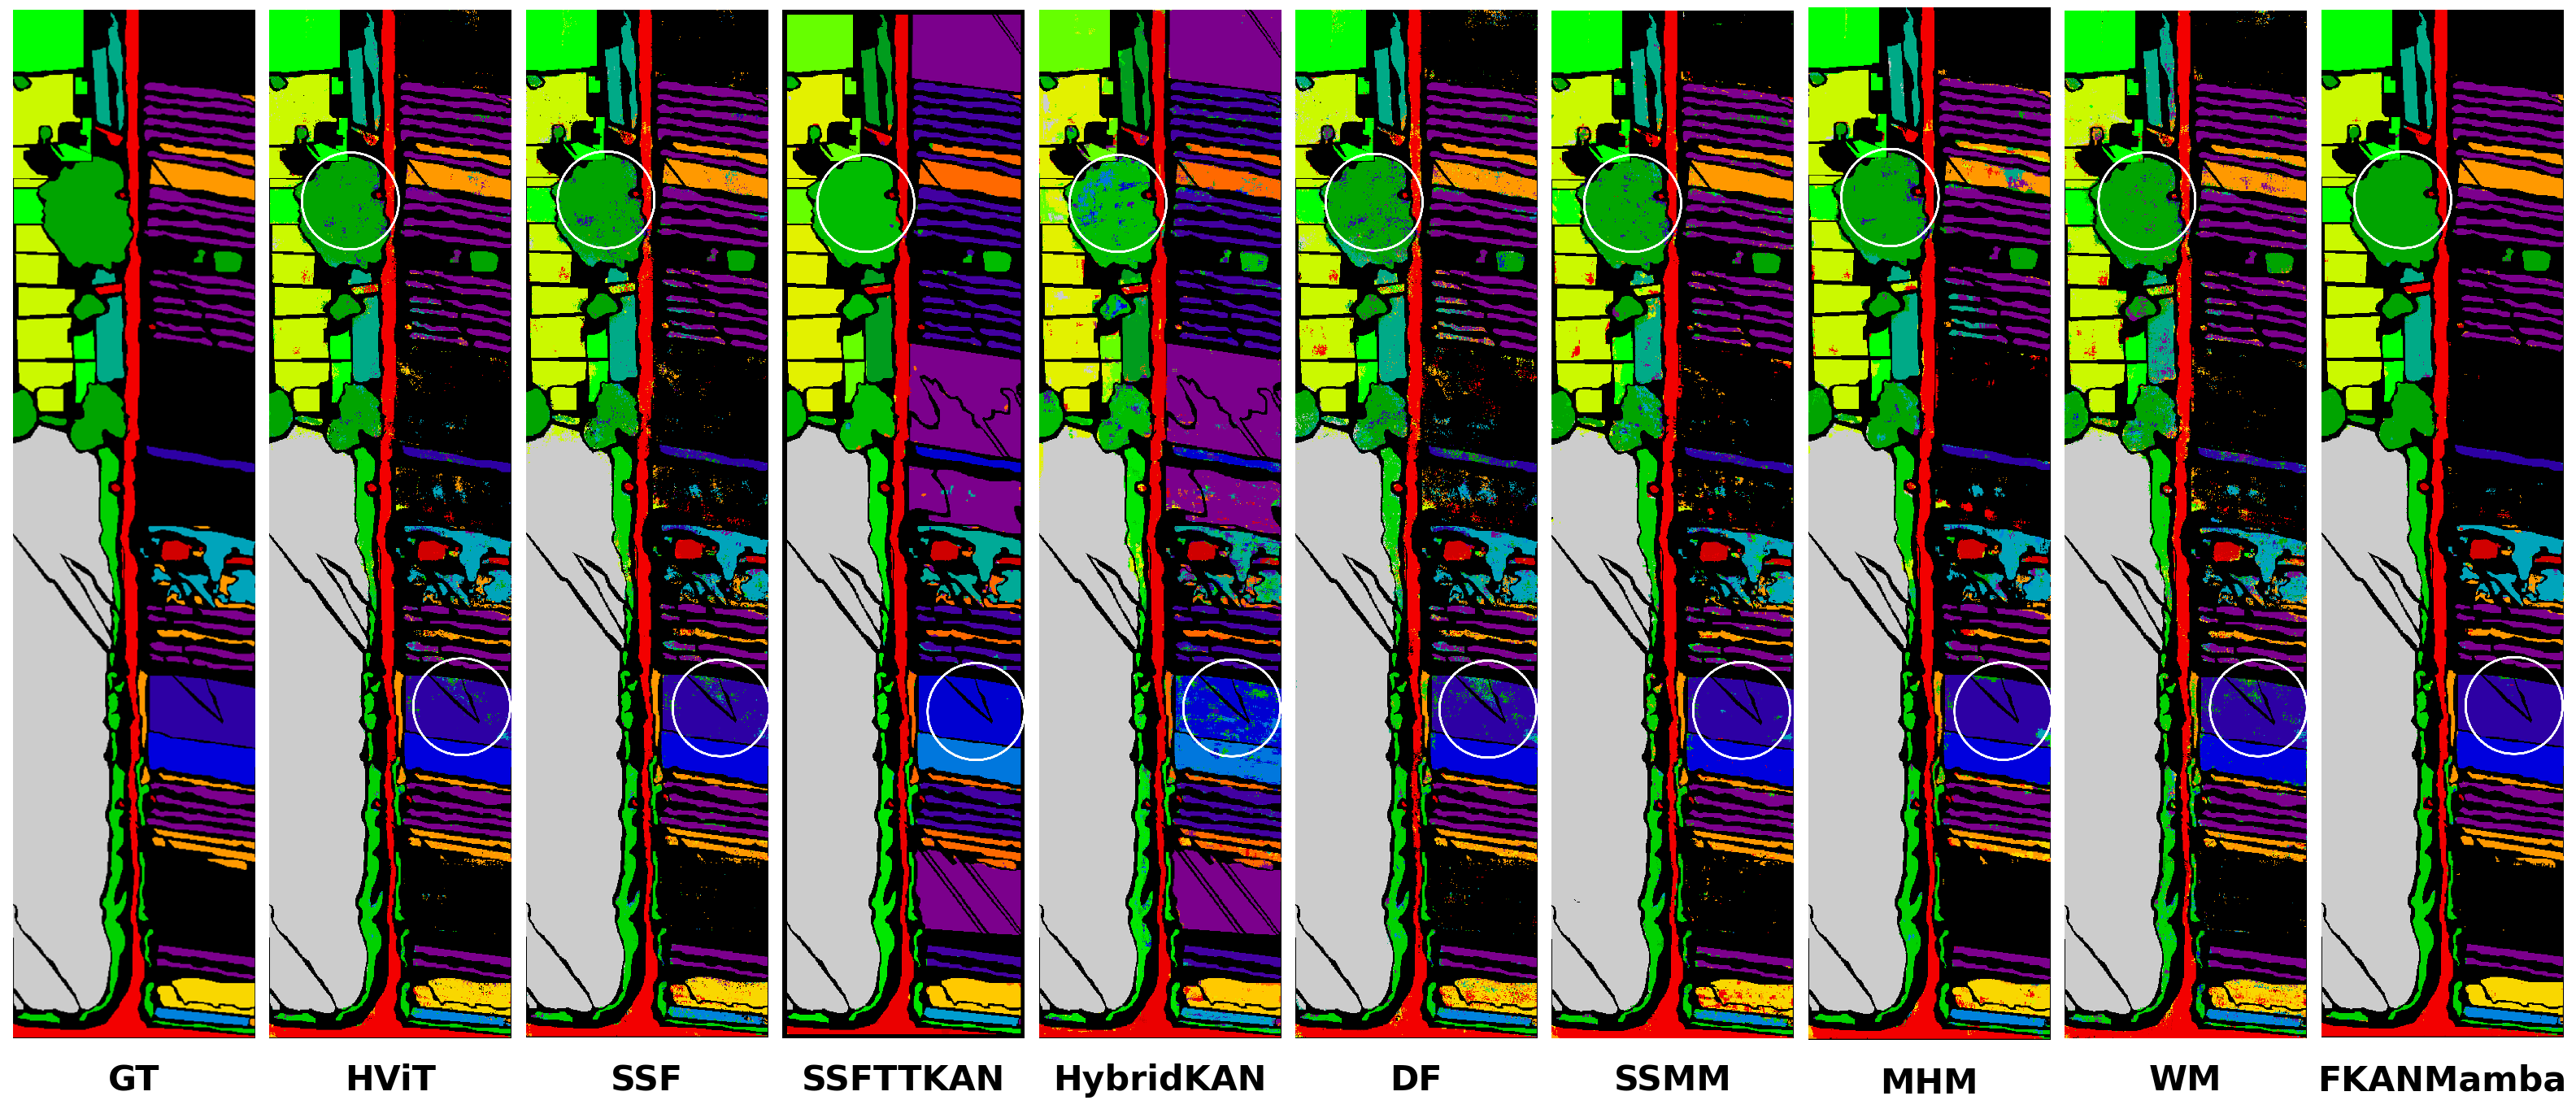
\includegraphics[width=0.98\textwidth]{revision_assets/figures/HC.png}
\caption{Historical within-scene classification maps on HC. External panel labels and layout have been revised for readability; predictions and class colors are unchanged.}
\label{fig:HC}
\end{figure*}
\begin{table}[!hbt]
    \centering
    \caption{Historical single-run within-scene results. Classwise and overall classification performance (\%) on HH dataset.}
    
    \resizebox{\columnwidth}{!}{\begin{tabular}{c|cccccccc|c} \hline 
        \textbf{Class} & \textbf{HViT} &\textbf{SSF} &\textbf{SSFTTKAN}  &\textbf{HybridKAN}  & \textbf{DF} & \textbf{SSMM} & \textbf{MHM}  & \textbf{WM} & \textbf{FKANMamba} \\ \hline
        Red roof  & 98.14 & 98.06 & 91.86 & 95.86 & \textcolor{orange}{\textbf{98.58}} & \textcolor{red}{\textbf{98.40}} & 97.08 & 93.35 & \textcolor{teal}{\textbf{98.67}} \\ 
        Road  & \textcolor{teal}{\textbf{95.50}} & 90.57 & \textcolor{red}{\textbf{90.98}} & \textcolor{orange}{\textbf{93.54}}  & 78.17 & 82.09 & 62.85 & 74.56 & 81.87 \\ 
        Bare soil  & 94.10 & 96.75 & 93.98 & \textcolor{orange}{\textbf{98.01}} & 92.63 & \textcolor{red}{\textbf{97.34}} & 94.28 & 84.11 & \textcolor{teal}{\textbf{99.48}} \\ 
        Cotton  & \textcolor{red}{\textbf{99.73}} & 99.64 & 97.59 & \textcolor{orange}{\textbf{99.76}}  & 99.00 & 99.72 & 98.91 & 98.10 & \textcolor{teal}{\textbf{99.84}} \\ 
        Cotton firewood  & 89.49 & 78.25 & \textcolor{teal}{\textbf{98.58}} & 92.24 & 77.05 & 90.27 & \textcolor{red}{\textbf{94.08}} & 68.29 & \textcolor{orange}{\textbf{96.55}} \\ 
        Rape   & 98.14 & 97.92 & \textcolor{teal}{\textbf{99.70}} & \textcolor{red}{\textbf{98.49}} & 97.22 & 97.92 & 96.86 & 98.28 & \textcolor{orange}{\textbf{99.13}} \\ 
        Chinese cabbage   & \textcolor{orange}{\textbf{96.57}} & 93.87 & \textcolor{red}{\textbf{96.40}} & 94.35  & 94.35 & 92.21 & 92.01 & 80.17 & \textcolor{teal}{\textbf{99.17}} \\ 
        Pakchoi    & 81.20 & 70.97 & \textcolor{teal}{\textbf{96.38}} & 75.11  & 65.66 & \textcolor{red}{\textbf{84.46}} & 65.25 & 58.89 & \textcolor{orange}{\textbf{87.33}} \\ 
        Cabbage   & \textcolor{teal}{\textbf{99.21}} & 97.57 & 98.22 & 97.43  & 96.62 & \textcolor{orange}{\textbf{98.63}} & 95.84 & 93.78 & \textcolor{red}{\textbf{98.30}} \\ 
        Tuber mustard  & 89.89 & 87.01 & \textcolor{red}{\textbf{93.07}} & \textcolor{orange}{\textbf{95.51}} & 85.06 & 92.77 & 85.34 & 75.42 & \textcolor{teal}{\textbf{98.01}} \\ 
        Brassica parachinensis & \textcolor{red}{\textbf{91.11}} & 89.00 & \textcolor{orange}{\textbf{95.53}} &  90.59 & 83.32 & 84.38 & 88.99 & 75.06 & \textcolor{teal}{\textbf{98.05}} \\ 
        Brassica chinensis     & 85.17 & 84.84 & \textcolor{orange}{\textbf{93.95}} &  \textcolor{red}{\textbf{89.16}} & 77.80 & 88.39 & 81.54 & 69.81 & \textcolor{teal}{\textbf{97.40}} \\ 
        Small Brassica chinensis  & 92.90 & 90.20 & \textcolor{teal}{\textbf{98.46}} & 93.14  & 87.23 & \textcolor{red}{\textbf{93.30}} & 83.79 & 76.36 & \textcolor{orange}{\textbf{98.43}} \\ 
        Lactuca sativa   & \textcolor{red}{\textbf{94.75}} & 93.09 & \textcolor{teal}{\textbf{98.61}} & 93.71 & 90.21 & 93.56 & 89.54 & 73.32 & \textcolor{orange}{\textbf{96.22}} \\ 
        Celtuce    & 89.80 & 86.03 &\textcolor{teal}{\textbf{97.22}} &\textcolor{red}{\textbf{93.34}}  & 87.58 & 91.01 & 80.37 & 42.68 & \textcolor{orange}{\textbf{95.34}}\\ 
        Film covered lettuce   & 94.53 & \textcolor{orange}{\textbf{ 99.34}} & \textcolor{red}{\textbf{99.20}} & 99.12 & 95.25 & 97.12 & 96.22 & 92.54 & \textcolor{teal}{\textbf{99.83}} \\ 
        Romaine lettuce     & 98.11 & 89.36 & \textcolor{orange}{\textbf{98.44}} & \textcolor{red}{\textbf{98.00}}  & 91.91 & 96.30 & 95.97 & 80.80 & \textcolor{teal}{\textbf{99.70}} \\ 
        Carrot   & 95.09 & \textcolor{orange}{\textbf{97.37}} & \textcolor{teal}{\textbf{98.79}} & 86.73 & 91.46 &96.68 & 95.75 & 82.38 & \textcolor{red}{\textbf{96.75}} \\ 
        White radish     & \textcolor{orange}{\textbf{94.69}} &  \textcolor{red}{\textbf{94.59}} & 94.14 & 92.22 & 92.43 & 92.50 & 90.74 & 87.27 & \textcolor{teal}{\textbf{97.23}} \\ 
        Garlic sprout   & \textcolor{red}{\textbf{93.97}} & 88.36 & \textcolor{teal}{\textbf{98.72}} & 87.02  & 74.94 & 91.32 & 86.03 & 75.67 & \textcolor{orange}{\textbf{96.20}} \\ 
        Broad bean       & \textcolor{orange}{\textbf{78.82}} & 58.99 & \textcolor{teal}{\textbf{97.07}} & 70.96  & 77.32 & 74.30 & 61.58 & 25.69 & \textcolor{red}{\textbf{78.32}} \\ 
        Tree   & 96.36 & \textcolor{red}{\textbf{97.02}} & \textcolor{teal}{\textbf{99.72}} & 95.32 & 86.60 & 95.40 & \textcolor{orange}{\textbf{97.41}} & 84.70 & 89.13 \\ \hline
        
        \textbf{OA (\%)}       & 96.72 & 95.83 & \textcolor{orange}{\textbf{97.09}} & \textcolor{red}{\textbf{96.81}}  & 94.15 & 96.45 & 94.30 & 89.69 & \textcolor{teal}{\textbf{98.63}} \\ 
        \textbf{AA (\%)}   &\textcolor{red}{\textbf{93.06}} & 89.95 & \textcolor{teal}{\textbf{96.66}}  & 92.26   & 87.29 & 92.19 & 87.75 & 76.87 & \textcolor{orange}{\textbf{95.50}} \\ 
        \textbf{$\kappa$}      & 95.86 & 94.72 & \textcolor{orange}{\textbf{96.34}} & \textcolor{red}{\textbf{95.97}} & 92.61 & 95.52 & 92.81 & 87.00 & \textcolor{teal}{\textbf{98.27}} \\ \hline
        
        \textbf{Param}    & \num{915158} &\num{2822550}  &\num {15063003} &\num{199547} & \num{224694} & \num{25052} & \num{23734} & \num{26710} & \num{37930} \\ \hline 
        % \textbf{Time (s)}   & 828 & 846 & 890 & \num{5128} & \num{3466} & \num{10598} & \num{2407} \\ \hline
    \end{tabular}}
    \label{tab:HH}
\end{table}











% \begin{table}[!hbt]
%     \centering
%     \caption{Classwise and overall classification performance (\%) on HH dataset.}
    
%     \resizebox{\columnwidth}{!}{\begin{tabular}{c|cccccccc|c} \hline 
%         \textbf{Class} & \textbf{HViT} &\textbf{SSFTTKAN}  &\textbf{HybridKAN} & \textbf{SSViT} & \textbf{DF} & \textbf{SSMM} & \textbf{MHM}  & \textbf{WM} & \textbf{FKANMamba} \\ \hline
%         Red roof   & 98.14 & 91.86 & 95.86 &\textcolor{teal}{\textbf{99.23}} & \textcolor{red}{\textbf{98.58}} & 98.40 & 97.08 & 93.35 & \textcolor{orange}{\textbf{98.67}} \\ 
%         Road  & \textcolor{teal}{\textbf{95.50}} & \textcolor{red}{\textbf{90.98}} & \textcolor{orange}{\textbf{93.54}} &83.58 & 78.17 & 82.09 & 62.85 & 74.56 & 81.87 \\ 
%         Bare soil  & 94.10 & 93.98 & \textcolor{orange}{\textbf{98.01}} & 96.35 & 92.63 & \textcolor{red}{\textbf{97.34}} & 94.28 & 84.11 & \textcolor{teal}{\textbf{99.48}} \\ 
%         Cotton  & 99.73 & 97.59 & \textcolor{red}{\textbf{99.76}} & \textcolor{orange}{\textbf{99.83}} & 99.00 & 99.72 & 98.91 & 98.10 & \textcolor{teal}{\textbf{99.84}} \\ 
%         Cotton firewood  & 89.49 & \textcolor{teal}{\textbf{98.58}} & 92.24 & 80.84 & 77.05 & 90.27 & \textcolor{red}{\textbf{94.08}} & 68.29 & \textcolor{orange}{\textbf{96.55}} \\ 
%         Rape   & 98.14 & \textcolor{teal}{\textbf{99.70}} & \textcolor{red}{\textbf{98.49}} & 97.61 & 97.22 & 97.92 & 96.86 & 98.28 & \textcolor{orange}{\textbf{99.13}} \\ 
%         Chinese cabbage   & \textcolor{orange}{\textbf{96.57}}& \textcolor{red}{\textbf{96.40}} & 94.35 & 95.38 & 94.35 & 92.21 & 92.01 & 80.17 & \textcolor{teal}{\textbf{99.17}} \\ 
%         Pakchoi    & 81.20 & \textcolor{teal}{\textbf{96.38}} & 75.11 & 75.82 & 65.66 & \textcolor{red}{\textbf{84.46}} & 65.25 & 58.89 & \textcolor{orange}{\textbf{87.33}} \\ 
%         Cabbage   & \textcolor{teal}{\textbf{99.21}} & 98.22 & 97.43 & \textcolor{orange}{\textbf{98.80}} & 96.62 & \textcolor{red}{\textbf{98.63}} & 95.84 & 93.78 & 98.30 \\ 
%         Tuber mustard  & 89.89 & 93.07 & \textcolor{orange}{\textbf{95.51}} & \textcolor{red}{\textbf{94.07}} & 85.06 & 92.77 & 85.34 & 75.42 & \textcolor{teal}{\textbf{98.01}} \\ 
%         Brassica parachinensis & 91.11 & \textcolor{orange}{\textbf{95.53}} &  90.59 &\textcolor{red}{\textbf{92.73}} & 83.32 & 84.38 & 88.99 & 75.06 & \textcolor{teal}{\textbf{98.05}} \\ 
%         Brassica chinensis     & 85.17 & \textcolor{red}{\textbf{93.95}} & 89.16 & \textcolor{red}{\textbf{92.96}} & 77.80 & 88.39 & 81.54 & 69.81 & \textcolor{teal}{\textbf{97.40}} \\ 
%         Small Brassica chinensis  & 92.90 & \textcolor{teal}{\textbf{98.46}} & 93.14  & 92.62 & 87.23 & \textcolor{red}{\textbf{93.30}} & 83.79 & 76.36 & \textcolor{orange}{\textbf{98.43}} \\ 
%         Lactuca sativa   & \textcolor{red}{\textbf{94.75}} & \textcolor{teal}{\textbf{98.61}} & 93.71 & 93.29 & 90.21 & 93.56 & 89.54 & 73.32 & \textcolor{orange}{\textbf{96.22}} \\ 
%         Celtuce    & 89.80 &\textcolor{teal}{\textbf{97.22}} & 93.34 &\textcolor{orange}{\textbf{95.45}} & 87.58 & 91.01 & 80.37 & 42.68 & \textcolor{red}{\textbf{95.34}}\\ 
%         Film covered lettuce   & 94.53 & \textcolor{orange}{\textbf{99.20}} & \textcolor{red}{\textbf{99.12}} & 95.14 & 95.25 & 97.12 & 96.22 & 92.54 & \textcolor{teal}{\textbf{99.83}} \\ 
%         Romaine lettuce     & 98.11 & \textcolor{orange}{\textbf{98.44}} & \textcolor{red}{\textbf{98.00}} & 96.12 & 91.91 & 96.30 & 95.97 & 80.80 & \textcolor{teal}{\textbf{99.70}} \\ 
%         Carrot   & 95.09 & \textcolor{teal}{\textbf{98.79}} & 86.73 & 91.95 & 91.46 & \textcolor{red}{\textbf{96.68}} & 95.75 & 82.38 & \textcolor{orange}{\textbf{96.75}} \\ 
%         White radish     & \textcolor{orange}{\textbf{94.69}} & \textcolor{red}{\textbf{94.14}} & 92.22 &94.13 & 92.43 & 92.50 & 90.74 & 87.27 & \textcolor{teal}{\textbf{97.23}} \\ 
%         Garlic sprout   & \textcolor{red}{\textbf{93.97}} & \textcolor{teal}{\textbf{98.72}} & 87.02 & 92.50 & 74.94 & 91.32 & 86.03 & 75.67 & \textcolor{orange}{\textbf{96.20}} \\ 
%         Broad bean       & \textcolor{orange}{\textbf{78.82}} & \textcolor{teal}{\textbf{97.07}} & 70.96  & 76.73 & 77.32 & 74.30 & 61.58 & 25.69 & \textcolor{red}{\textbf{78.32}} \\ 
%         Tree   & \textcolor{red}{\textbf{96.36}} & \textcolor{teal}{\textbf{99.72}} & 95.32 & 94.38 & 86.60 & 95.40 & \textcolor{orange}{\textbf{97.41}} & 84.70 & 89.13 \\ \hline
        
%         \textbf{OA (\%)}       & 96.72 & \textcolor{orange}{\textbf{97.09}} & \textcolor{red}{\textbf{96.81}} & 96.73 & 94.15 & 96.45 & 94.30 & 89.69 & \textcolor{teal}{\textbf{98.63}} \\ 
%         \textbf{AA (\%)}   &\textcolor{red}{\textbf{93.06}} & \textcolor{teal}{\textbf{96.66}}  & 92.26 & 92.25  & 87.29 & 92.19 & 87.75 & 76.87 & \textcolor{orange}{\textbf{95.50}} \\ 
%         \textbf{$\kappa$}      &95.86 & \textcolor{orange}{\textbf{96.34}} & \textcolor{red}{\textbf{95.97}} & 95.86  & 92.61 & 95.52 & 92.81 & 87.00 & \textcolor{teal}{\textbf{98.27}} \\ \hline
        
%         \textbf{Param}    & \num{915158}  &\num {15063003} &\num{199547} &\num{915158} & \num{224694} & \num{25052} & \num{23734} & \num{26710} & \num{37930} \\ \hline 
%         % \textbf{Time (s)}   & 828 & 846 & 890 & \num{5128} & \num{3466} & \num{10598} & \num{2407} \\ \hline
%     \end{tabular}}
%     \label{tab:HH}
% \end{table}


\begin{revision}
Table~\ref{tab:HH} and Fig.~\ref{fig:HH} show the historical HH within-scene results. These scores are single-run observations under overlapping random-pixel sampling and full-scene PCA. They establish neither repeated-run superiority nor spatially independent generalization. The reported OA difference between FKANMamba and SSF is $98.63-95.83=2.80$ percentage points. SSFTTKAN has higher AA, so the table does not show uniform superiority across metrics. Parameter counts measure storage size; the maps are qualitative illustrations rather than independent evidence of deployment performance.
\end{revision}

\begin{figure*}[t]
\centering
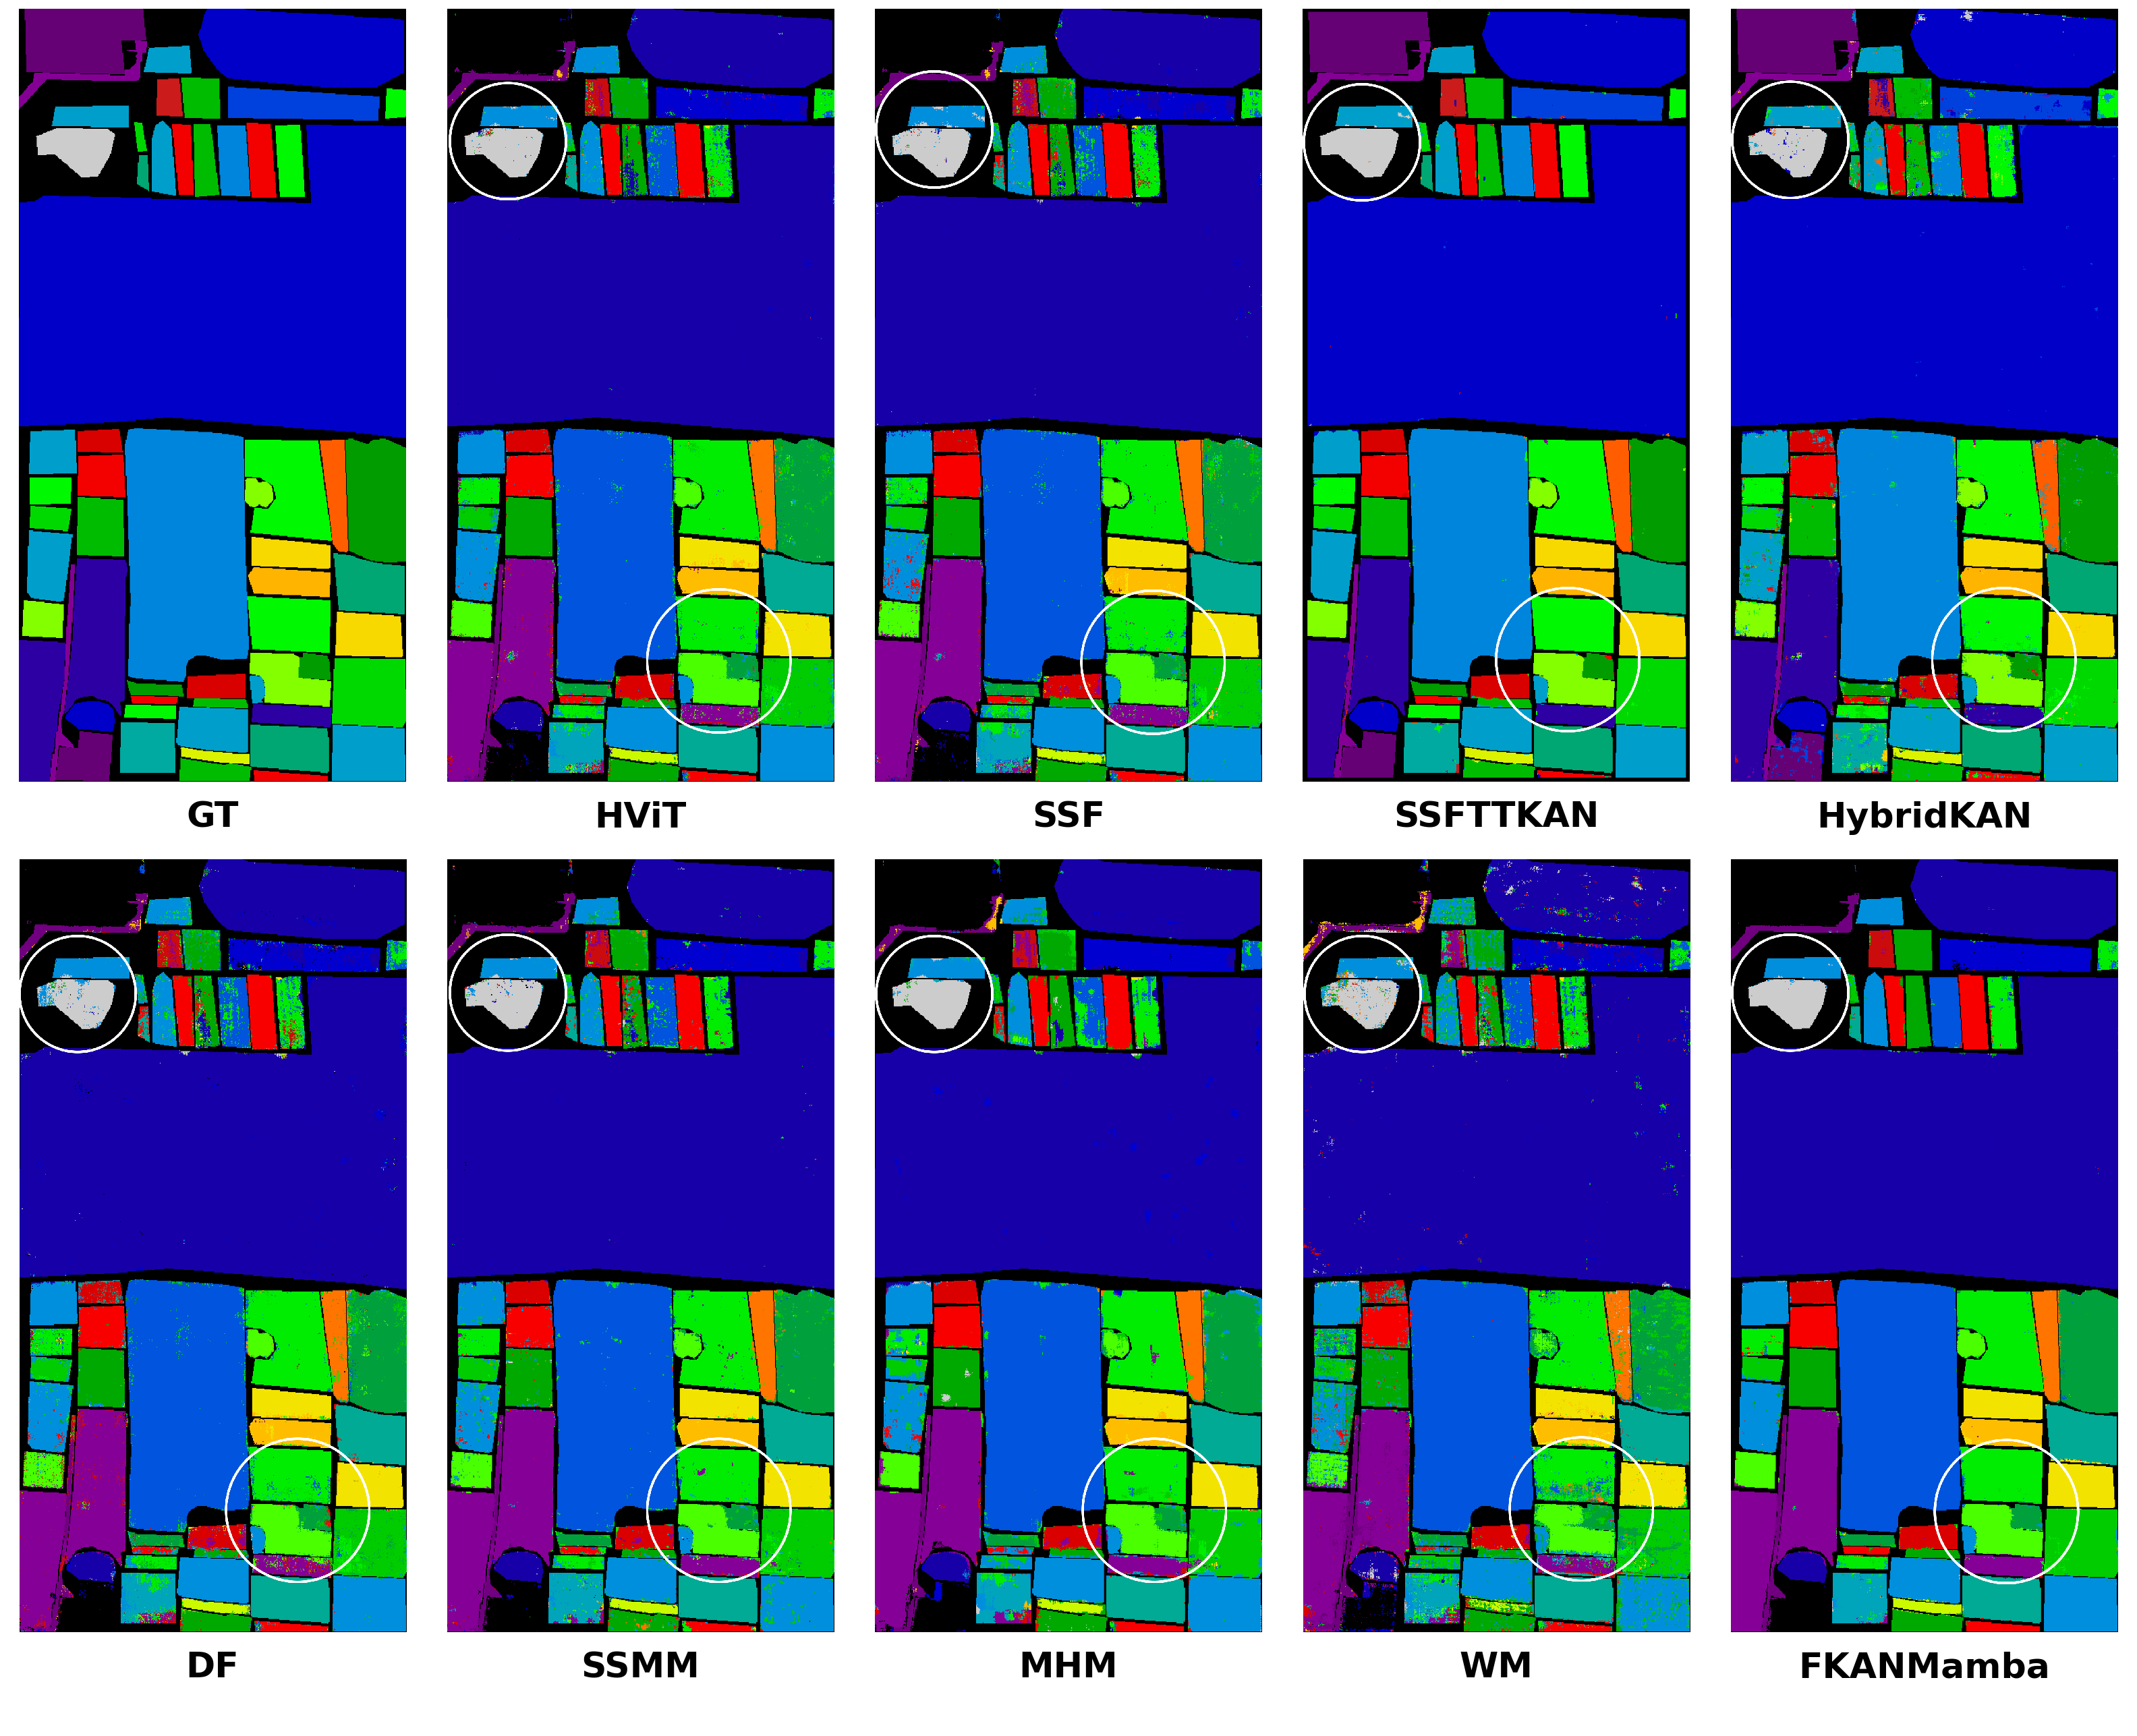
\includegraphics[width=0.98\textwidth]{revision_assets/figures/HH.png}
\caption{Historical within-scene classification maps on HH. External panel labels and layout have been revised for readability; predictions and class colors are unchanged.}
\label{fig:HH}
\end{figure*}

\begin{revision}
Table~\ref{tab:TH} and Fig.~\ref{fig:TH} show the historical TH within-scene results. These scores are single-run observations under overlapping random-pixel sampling and full-scene PCA. They establish neither repeated-run superiority nor spatially independent generalization. Parameter counts measure storage size; the maps are qualitative illustrations rather than independent evidence of deployment performance.
\end{revision}

\begin{table}[!hbt]
\centering
    \caption{Historical single-run within-scene results. Classwise and overall classification performance (\%) on TH dataset.}
    
    \resizebox{\columnwidth}{!}{\begin{tabular}{c|cccccccc|c} \hline
        \textbf{Class}  & \textbf{HViT} & \textbf{SSF} & \textbf{SSFTTKAN} & \textbf{HybridKAN}  & \textbf{DF} & \textbf{SSMM} & \textbf{MHM}  & \textbf{WM} & \textbf{FKANMamba} \\ \hline
        Rubber track  & \textcolor{red}{\textbf{99.93}} & 99.92 & 99.19 & 99.57 & \textcolor{orange}{\textbf{99.96}} & 99.86 & 99.90 & 99.12 & \textcolor{teal}{\textbf{99.97}} \\ 
        Flagging   & \textcolor{orange}{\textbf{99.45}} & 99.05 & 98.22 & 98.45 & \textcolor{red}{\textbf{99.12}} & 98.61 & 99.01 & 98.93 & \textcolor{teal}{\textbf{99.49}} \\ 
        Sandy   & \textcolor{orange}{\textbf{98.15}} & 94.97 & 90.57 & 96.01 & \textcolor{red}{\textbf{98.11}} & 88.63 & 96.48 & 94.26 & \textcolor{teal}{\textbf{98.70}} \\ 
        Asphalt & \textcolor{red}{\textbf{99.68}} & \textcolor{orange}{\textbf{99.74}} & 99.27 & 99.36 & 99.54 & 98.58 & 99.50 & 98.57 & \textcolor{teal}{\textbf{99.91}} \\ 
        Boardwalk & \textcolor{red}{\textbf{96.83}} & 96.24 & \textcolor{teal}{\textbf{99.88}} & 82.51  & 94.74 & 60.02 & 93.37 & 82.33 & \textcolor{orange}{\textbf{97.37}} \\ 
        Rocky shallows   & \textcolor{teal}{\textbf{98.47}} & \textcolor{red}{\textbf{98.15}} & 96.30 & 92.76  & 91.38 & 94.05 & 93.32 & 94.38 & \textcolor{orange}{\textbf{98.39}} \\ 
        Grassland   & \textcolor{red}{\textbf{93.66}} & 86.96 & \textcolor{orange}{\textbf{93.78}} & 83.38  & 91.71 & 72.67 & 89.43 & 89.39 &\textcolor{teal}{\textbf{95.79}} \\ 
        Bulrush   & \textcolor{teal}{\textbf{100}} & \textcolor{orange}{\textbf{99.99}} & 96.71 & 99.96  & \textcolor{red}{\textbf{99.96}} & 99.87 & 99.83 & 99.95 & \textcolor{teal}{\textbf{100}} \\ 
        Gravel road & \textcolor{orange}{\textbf{99.89}} & \textcolor{red}{\textbf{99.74}} & \textcolor{teal}{\textbf{99.91}} & 99.43  & 99.46 & 97.96 & 99.25 & 98.62 & 99.68 \\ 
        Ligustrum vicaryi  & \textcolor{teal}{\textbf{99.81}} & 91.09 &\textcolor{orange}{\textbf{99.25}} & 85.42  & 96.19 & 90.09 & 54.57 & 91.77 & \textcolor{red}{\textbf{95.38}} \\ 
        Coniferous pine & \textcolor{red}{\textbf{98.72}} & 94.07 & \textcolor{teal}{\textbf{99.36}} & 70.58  & 95.05 & 87.53 & 96.26 & 92.94 & \textcolor{orange}{\textbf{99.20}} \\ 
        Spiraea   & 86.49 &\textcolor{red}{\textbf{98.96}} & 98.96 & 85.75  & 82.19 & 88.13 & \textcolor{teal}{\textbf{99.40}} & 81.75 & \textcolor{orange}{\textbf{99.10}} \\ 
        Bare soil  & \textcolor{teal}{\textbf{100}} & \textcolor{orange}{\textbf{99.86}} & \textcolor{red}{\textbf{99.47}} & 99.27  & 99.86 & 93.80 & 99.07 & 98.02 &\textcolor{teal}{\textbf{100}} \\ 
        Buxus sinica  & \textcolor{teal}{\textbf{99.74}} & 81.93 &\textcolor{orange}{\textbf{99.49}} & 90.33  & 96.36 & 82.93 & 79.17 & 82.93 & \textcolor{red}{\textbf{98.36}} \\ 
        Photinia serrulata  & \textcolor{orange}{\textbf{95.96}} & 91.34 & \textcolor{teal}{\textbf{97.68}} & 86.89 & 95.00 & 85.00 & 93.44 & 90.18 & \textcolor{red}{\textbf{95.55}} \\  
        Populus & 98.09 & 97.88 & \textcolor{orange}{\textbf{98.77}} & 96.49  & 96.66 & 96.68 & 97.74 & \textcolor{red}{\textbf{98.25}} & \textcolor{teal}{\textbf{99.65}} \\ 
        Ulmus pumila L   & \textcolor{red}{\textbf{97.60}} & \textcolor{orange}{\textbf{98.49}} & \textcolor{teal}{\textbf{98.90}} & 92.82 & 95.46 & 92.12 & 96.36 & 88.51 &96.49 \\ 
        Seawater & 99.95 &\textcolor{orange}{\textbf{99.97}}  & 95.79 & \textcolor{red}{\textbf{99.96}} & 99.93 & 99.93 & 99.88 & 99.75 & \textcolor{teal}{\textbf{99.99}} \\ \hline
        
        \textbf{OA (\%)}      & \textcolor{orange}{\textbf{98.81}} & \textcolor{red}{\textbf{ 98.02}} & 97.60 & 95.96 & 97.62 & 95.73 & 97.70 & 97.30 & \textcolor{teal}{\textbf{99.31}} \\ 
        \textbf{AA (\%)}     & \textcolor{orange}{\textbf{97.91}} & 96.02  &  \textcolor{red}{\textbf{97.86}} & 92.16  & 96.15 & 90.36 & 93.67 & 93.31 & \textcolor{teal}{\textbf{98.50}} \\ 
        \textbf{$\kappa$}    & \textcolor{orange}{\textbf{98.65}} &  \textcolor{red}{\textbf{97.74}} & 97.28 & 95.40  & 97.30 & 95.13 & 97.38 & 96.92 & \textcolor{teal}{\textbf{99.21}} \\\hline
        
        \textbf{Parameters} & \num{914130}  &\num{2821522} & \num{15062743} & \num{198391}  & \num{224562} & \num{24536} & \num{23218} & \num{26194} & \num{37670} \\ \hline
        % \textbf{Time (s)}  & \num{603} & \num{1001} & \num{566} & \num{7036} & \num{4887} & \num{15984} & \num{6400} \\ \hline
    \end{tabular}}
    \label{tab:TH}
\end{table}



\begin{figure*}[t]
\centering
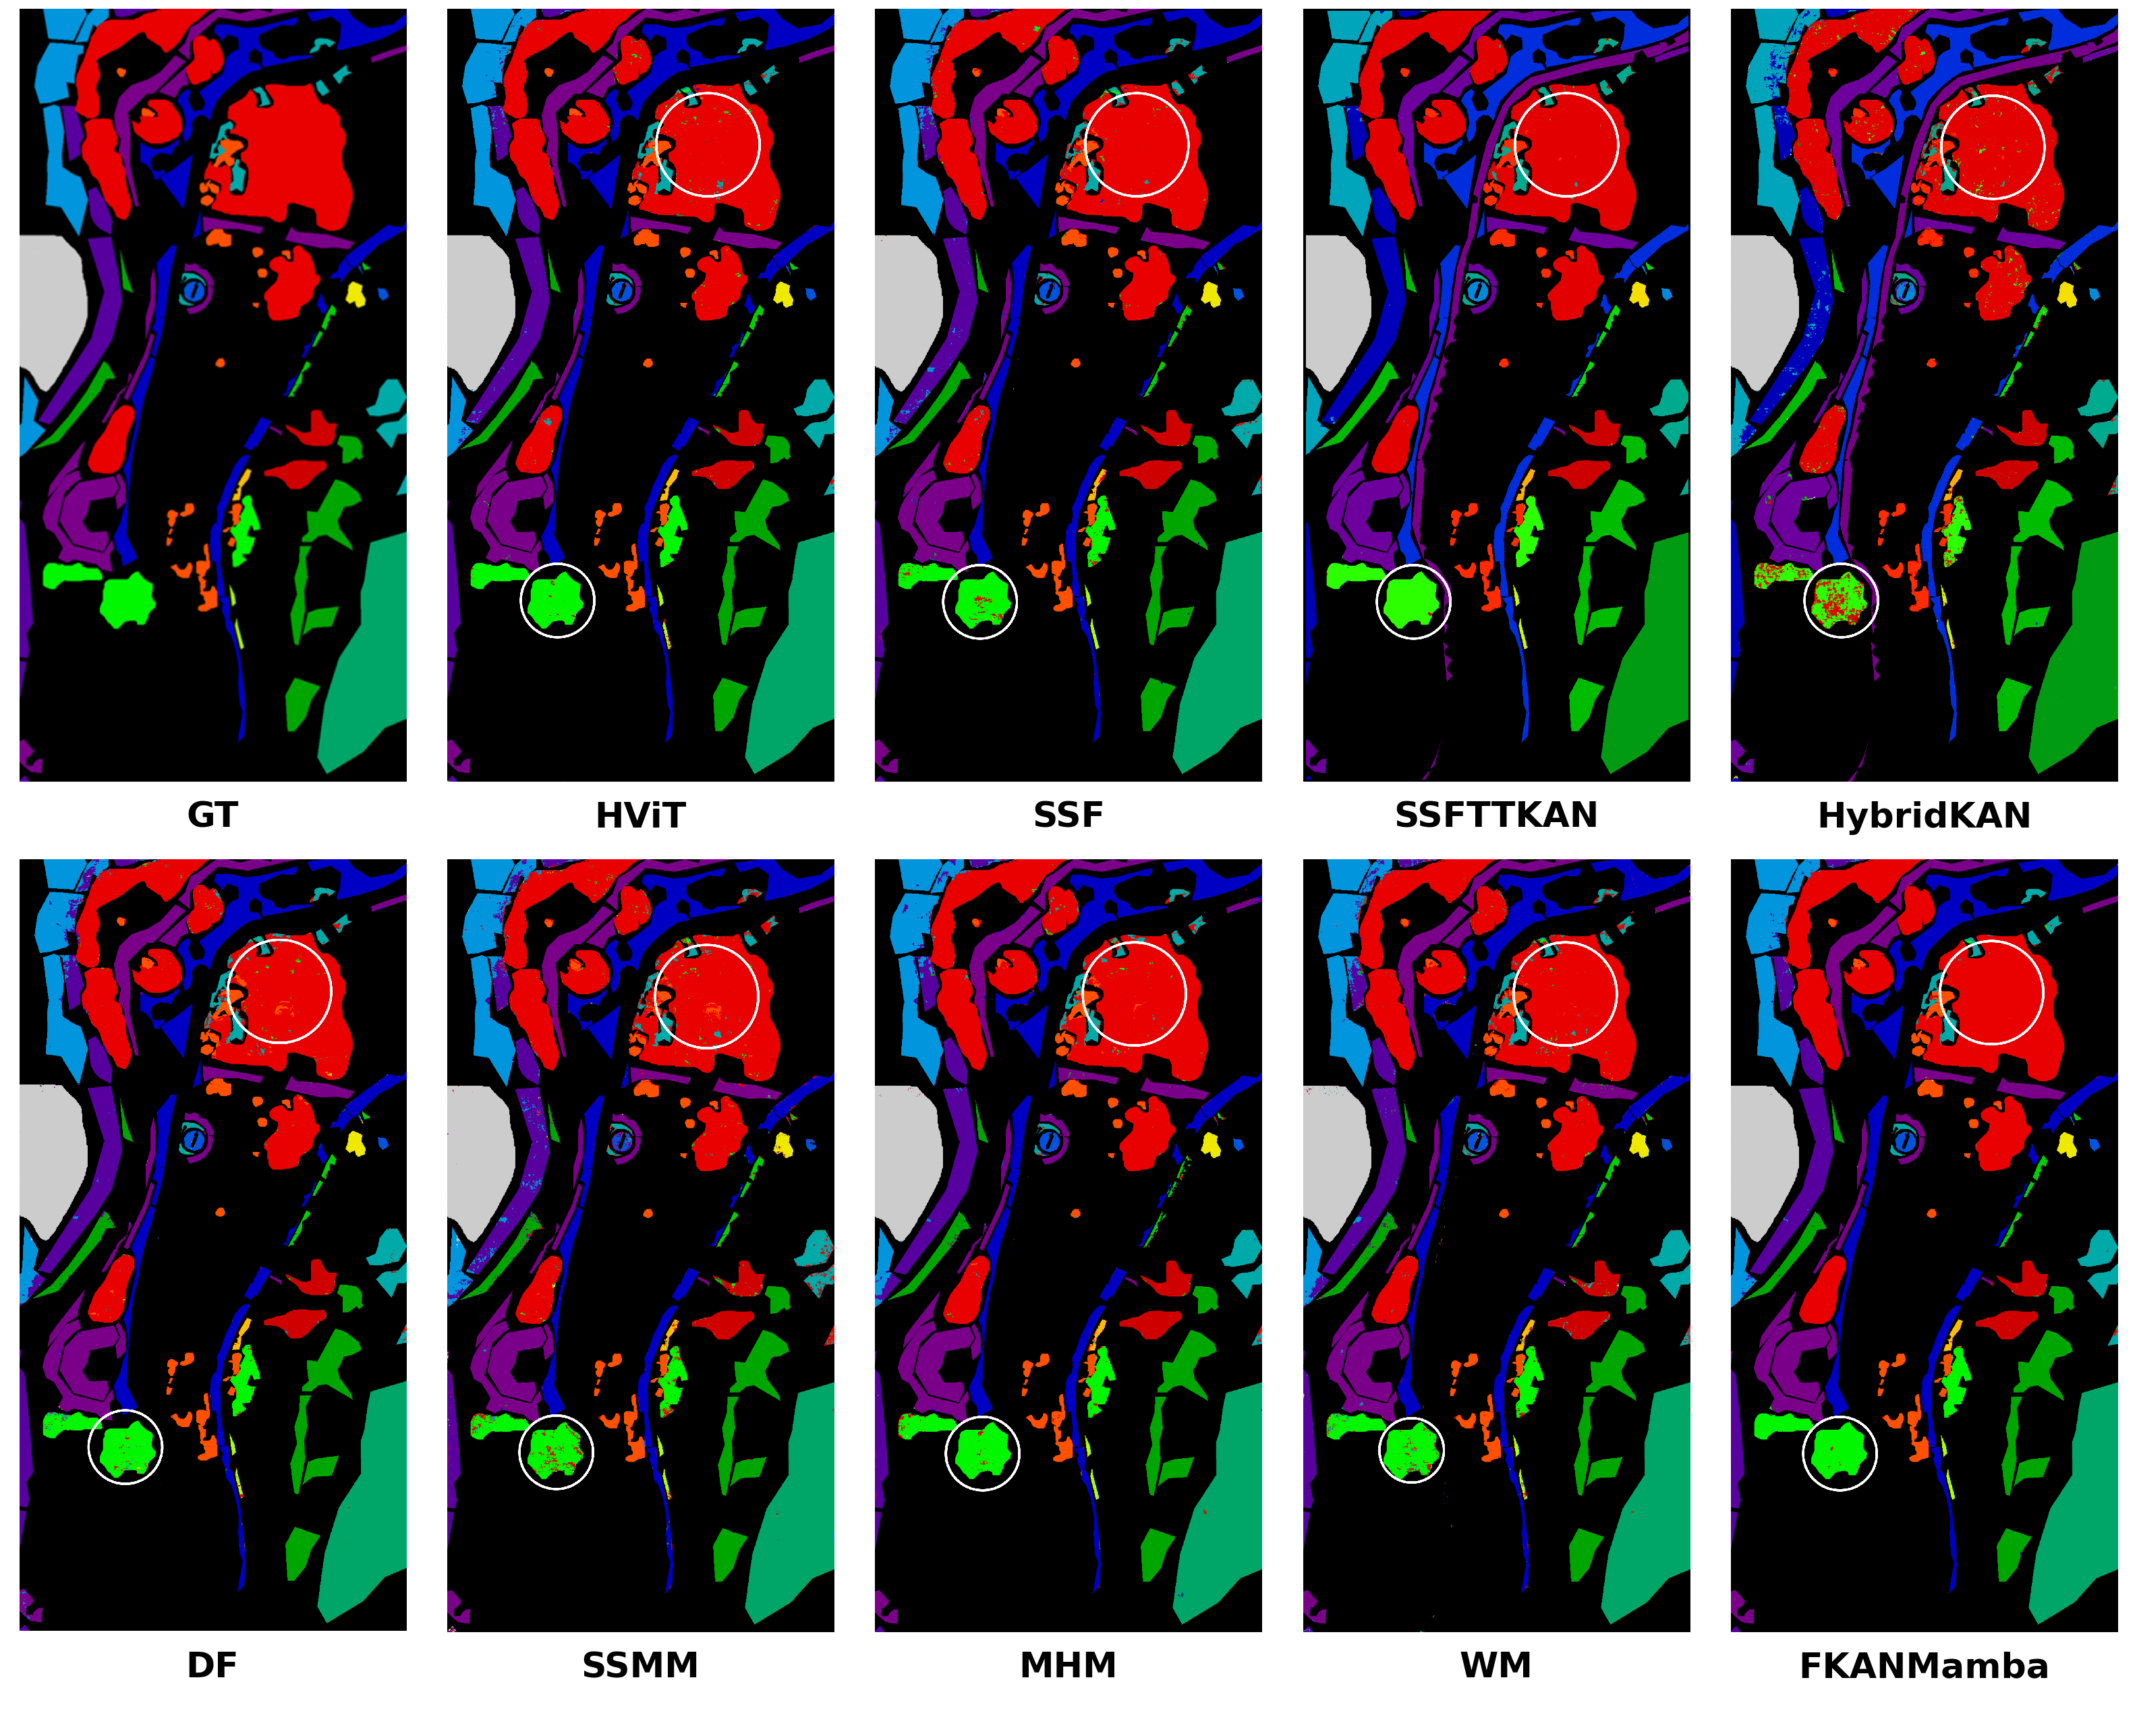
\includegraphics[width=0.98\textwidth]{revision_assets/figures/TH.png}
\caption{Historical within-scene classification maps on TH. External panel labels and layout have been revised for readability; predictions and class colors are unchanged.}
\label{fig:TH}
\end{figure*}

\begin{revision}
Table~\ref{tab:PI} and Fig.~\ref{fig:PI} show the historical PI within-scene results. These scores are single-run observations under overlapping random-pixel sampling and full-scene PCA. They establish neither repeated-run superiority nor spatially independent generalization. Parameter counts measure storage size; the maps are qualitative illustrations rather than independent evidence of deployment performance.
\end{revision}

\begin{table}[!hbt]
\centering
\caption{Historical single-run within-scene results. Classwise and overall classification performance (\%) on PI dataset.}

\resizebox{\columnwidth}{!}{\begin{tabular}{c|cccccccc|c} \hline
            \textbf{Class}  & \textbf{HViT} & \textbf{SSF} & \textbf{SSFTTKAN} & \textbf{HybridKAN} & \textbf{DF} & \textbf{SSMM} & \textbf{MHM} & \textbf{WM} & \textbf{FKANMamba} \\ \hline
            Ship  & \textcolor{red}{\textbf{90.81}} & 92.35 & \textcolor{orange}{\textbf{94.77}} & 88.16  & 90.42 & 83.33 & 88.12 & 89.99 & \textcolor{teal}{\textbf{94.84}}\\ 
            Seawater    & \textcolor{teal}{\textbf{99.55}} & \textcolor{orange}{\textbf{99.39}} & 98.33 & 99.28  & 99.04 & 98.84 & 99.23 & 98.78 & \textcolor{red}{\textbf{99.36}} \\ 
            Trees  & \textcolor{orange}{\textbf{97.90}} & \textcolor{red}{\textbf{96.87 }}& 90.79 & 93.12 & 97.62 & 88.72 & \textcolor{teal}{\textbf{99.14}} & 96.53 & 93.07 \\ 
            Concrete structure building  & \textcolor{teal}{\textbf{98.79}} & 97.64 & \textcolor{red}{\textbf{97.73}} & 94.83  & 96.06 & 91.69 & 96.06 & 94.70 & \textcolor{orange}{\textbf{98.04}} \\ 
            Floating pier  & \textcolor{orange}{\textbf{96.70}} & 94.61 &  \textcolor{teal}{\textbf{98.61}}  & 87.81  & 90.15 & 83.20 & 85.49 & 85.94 & \textcolor{red}{\textbf{96.33}} \\ 
            Brick houses   & \textcolor{teal}{\textbf{99.29}} & \textcolor{red}{\textbf{97.22}} & 91.43 & 93.63  & 95.90 & 90.66 & 97.19 & 91.00 & \textcolor{orange}{\textbf{98.61}} \\ 
            Steel houses   & 97.69 & \textcolor{orange}{\textbf{98.41}} & \textcolor{teal}{\textbf{98.88}} & 97.14  & 96.64 & 87.68 & 96.76 & 80.46 & \textcolor{red}{\textbf{97.72}}\\ 
            Wharf construction land  & \textcolor{red}{\textbf{95.60}} & 95.19 & 95.28 & 94.94  & 95.23 & 92.18 & \textcolor{orange}{\textbf{96.74}} & 94.03 & \textcolor{teal}{\textbf{99.25}} \\ 
            Car   & \textcolor{red}{\textbf{90.48}} & 89.43 &\textcolor{teal}{\textbf{95.29}} & 79.96  & 79.08 & 51.89 & 82.29 & 35.85 & \textcolor{orange}{\textbf{92.87}}\\ 
            Road  & \textcolor{orange}{\textbf{99.14}} & \textcolor{red}{\textbf{99.00}} & 96.70 & 97.98 & 98.40 & 95.62 & 98.23 & 98.27 & \textcolor{teal}{\textbf{99.19}} \\ \hline
            
            \textbf{OA (\%)}  & \textcolor{orange}{\textbf{98.58}} & \textcolor{red}{\textbf{98.33}} & 97.36 & 97.34 & 97.62 & 95.42 & 97.65 & 96.60 &  \textcolor{teal}{\textbf{98.84}} \\ 
            \textbf{AA (\%)}    & \textcolor{orange}{\textbf{96.60}}& \textcolor{red}{\textbf{96.01}}  & 95.78 & 92.69 & 93.85 & 86.38 & 93.92 & 86.55 &  \textcolor{teal}{\textbf{96.93}}\\ 
            \textbf{$\kappa$} & \textcolor{orange}{\textbf{97.88}} & \textcolor{red}{\textbf{97.52}} & 96.10 & 96.03 & 96.46 & 93.18 & 96.50 & 94.92 &  \textcolor{teal}{\textbf{98.27}} \\ \hline
            
            \textbf{Param} & \num{912074} &\num{2819466} & \num{15062223} &\num{196079} & \num{224298} & \num{23504} & \num{22186} & \num{25162} & \num{37150} \\ \hline
            % \textbf{Time (s)}  & \num{2094} & \num{2089} & \num{2529} & \num{14925} & \num{9598} & \num{20717} & \num{12993} \\ \hline
    \end{tabular}}
    \label{tab:PI}
\end{table}











% \begin{table}[!hbt]
% \centering
% \caption{Classwise and overall classification performance (\%) on Pingan dataset.}

% \resizebox{\columnwidth}{!}{\begin{tabular}{c|cccccccc|c} \hline
%             \textbf{Class}  & \textbf{HViT} & \textbf{SSFTTKAN} & \textbf{HybridKAN} & \textbf{SSViT} & \textbf{DF} & \textbf{SSMM} & \textbf{MHM} & \textbf{WM} & \textbf{FKANMamba} \\ \hline
%             Ship  & \textcolor{red}{\textbf{90.81}} & \textcolor{orange}{\textbf{94.77}} & 88.16 & 90.46 & 90.42 & 83.33 & 88.12 & 89.99 & \textcolor{teal}{\textbf{94.84}}\\ 
%             Seawater    & \textcolor{teal}{\textbf{99.55}} & 98.33 & 99.28 & \textcolor{orange}{\textbf{99.51}} & 99.04 & 98.84 & 99.23 & 98.78 & \textcolor{red}{\textbf{99.36}} \\ 
%             Trees  & \textcolor{red}{\textbf{97.90}} & 90.79 & 93.12 & \textcolor{teal}{\textbf{99.66}} & 97.62 & 88.72 & \textcolor{orange}{\textbf{99.14}} & 96.53 & 93.07 \\ 
%             Concrete structure building  & \textcolor{teal}{\textbf{98.79}} & 97.73 & 94.83 & \textcolor{orange}{\textbf{98.70}} & 96.06 & 91.69 & 96.06 & 94.70 & \textcolor{red}{\textbf{98.04}} \\ 
%             Floating pier        & \textcolor{red}{\textbf{96.70}} &  \textcolor{teal}{\textbf{98.61}}  & 87.81 &\textcolor{orange}{\textbf{96.71}} & 90.15 & 83.20 & 85.49 & 85.94 & 96.33 \\ 
%             Brick houses      & \textcolor{teal}{\textbf{99.29}} & 91.43 & 93.63 & \textcolor{red}{\textbf{98.42}} & 95.90 & 90.66 & 97.19 & 91.00 & \textcolor{orange}{\textbf{98.61}} \\ 
%             Steel houses     & 97.69 & \textcolor{teal}{\textbf{98.88}} & 97.14 & \textcolor{orange}{\textbf{98.41}} & 96.64 & 87.68 & 96.76 & 80.46 & \textcolor{red}{\textbf{97.72}}\\ 
%             Wharf construction land  & 95.60 & 95.28 & 94.94 & \textcolor{orange}{\textbf{98.23}} & 95.23 & 92.18 & \textcolor{red}{\textbf{96.74}} & 94.03 & \textcolor{teal}{\textbf{99.25}} \\ 
%             Car   & 90.48 &\textcolor{teal}{\textbf{95.29}} & 79.96 & \textcolor{red}{\textbf{91.10}} & 79.08 & 51.89 & 82.29 & 35.85 & \textcolor{orange}{\textbf{92.87}}\\ 
%             Road  & \textcolor{orange}{\textbf{99.14}} & 96.70 & 97.98 &\textcolor{red}{\textbf{98.81}} & 98.40 & 95.62 & 98.23 & 98.27 & \textcolor{teal}{\textbf{99.19}} \\ \hline
            
%             \textbf{OA (\%)}  & \textcolor{red}{\textbf{98.58}} & 97.36 & 97.34 &\textcolor{orange}{\textbf{98.66}} & 97.62 & 95.42 & 97.65 & 96.60 &  \textcolor{teal}{\textbf{98.84}} \\ 
%             \textbf{AA (\%)}    & \textcolor{red}{\textbf{96.60}} & 95.78 & 92.69 & \textcolor{teal}{\textbf{97.00}} & 93.85 & 86.38 & 93.92 & 86.55 &  \textcolor{orange}{\textbf{96.93}}\\ 
%             \textbf{$\kappa$} & \textcolor{red}{\textbf{97.88}} & 96.10 & 96.03 & \textcolor{orange}{\textbf{98.00}} & 96.46 & 93.18 & 96.50 & 94.92 &  \textcolor{teal}{\textbf{98.27}} \\ \hline
            
%             \textbf{Param} & \num{912074} & \num{15062223} &\num{196079} &\num{912074} & \num{224298} & \num{23504} & \num{22186} & \num{25162} & \num{37150} \\ \hline
%             % \textbf{Time (s)}  & \num{2094} & \num{2089} & \num{2529} & \num{14925} & \num{9598} & \num{20717} & \num{12993} \\ \hline
%     \end{tabular}}
%     \label{tab:PI}
% \end{table}





% \begin{table}[!hbt]
% \centering
% \caption{Classwise and overall classification performance (\%) on Pingan dataset.}
% \label{tab:PI}
% \resizebox{\columnwidth}{!}{\begin{tabular}{c|ccccccc|c} \hline
%             \textbf{Class}  & \textbf{HViT} & \textbf{SSFTTKAN} & \textbf{SSViT} & \textbf{DF} & \textbf{SSMM} & \textbf{MHM} & \textbf{WM} & \textbf{FKANMamba} \\ \hline
%             Ship   & \textcolor{orange}{\textbf{90.81}} & 94.80 & \textcolor{red}{\textbf{90.46}} & 90.42 & 83.33 & 88.12 & 89.99 & \textcolor{teal}{\textbf{94.84}}\\ 
%             Seawater    & \textcolor{teal}{\textbf{99.55}} & 98.27 & \textcolor{orange}{\textbf{99.51}} & 99.04 & 98.84 & 99.23 & 98.78 & \textcolor{red}{\textbf{99.36}} \\ 
%             Trees  & \textcolor{red}{\textbf{97.90}} &90.63 & \textcolor{teal}{\textbf{99.66}} & 97.62 & 88.72 & \textcolor{orange}{\textbf{99.14}} & 96.53 & 93.07 \\ 
%             Concrete structure building  & \textcolor{teal}{\textbf{98.79}} &97.72 & \textcolor{orange}{\textbf{98.70}} & 96.06 & 91.69 & 96.06 & 94.70 & \textcolor{red}{\textbf{98.04}} \\ 
%             Floating pier               & \textcolor{orange}{\textbf{96.70}} & 98.81 &\textcolor{teal}{\textbf{96.71}} & 90.15 & 83.20 & 85.49 & 85.94 & \textcolor{red}{\textbf{96.33}} \\ 
%             Brick houses                & \textcolor{teal}{\textbf{99.29}} &91.04 &\textcolor{red}{\textbf{98.42}} & 95.90 & 90.66 & 97.19 & 91.00 & \textcolor{orange}{\textbf{98.61}} \\ 
%             Steel houses                & \textcolor{red}{\textbf{97.69}} & 99.03 &\textcolor{teal}{\textbf{98.41}} & 96.64 & 87.68 & 96.76 & 80.46 & \textcolor{orange}{\textbf{97.72 }}\\ 
%             Wharf construction land     & 95.60 & 95.19 &\textcolor{orange}{\textbf{98.23}} & 95.23 & 92.18 & \textcolor{red}{\textbf{96.74}} & 94.03 & \textcolor{teal}{\textbf{99.25}} \\ 
%             Car    & \textcolor{red}{\textbf{90.48}} & 94.49 &\textcolor{orange}{\textbf{91.10}} & 79.08 & 51.89 & 82.29 & 35.85 & \textcolor{teal}{\textbf{92.87}}\\ 
%             Road   & \textcolor{orange}{\textbf{99.14}} & 96.71 &\textcolor{red}{\textbf{98.81}} & 98.40 & 95.62 & 98.23 & 98.27 & \textcolor{teal}{\textbf{99.19}} \\ \hline
%             \textbf{OA (\%)}  & \textcolor{red}{\textbf{98.58}} & 97.32 &\textcolor{orange}{\textbf{98.66}} & 97.62 & 95.42 & 97.65 & 96.60 &  \textcolor{teal}{\textbf{98.84}} \\ 
%             \textbf{AA (\%)}    & \textcolor{red}{\textbf{96.60}} & 95.67 & \textcolor{orange}{\textbf{97.00}} & 93.85 & 86.38 & 93.92 & 86.55 &  \textcolor{teal}{\textbf{96.93}}\\ 
%             \textbf{$\kappa$}            & \textcolor{red}{\textbf{97.88}} &96.04 & \textcolor{orange}{\textbf{98.00}} & 96.46 & 93.18 & 96.50 & 94.92 &  \textcolor{teal}{\textbf{98.27}} \\ \hline
%             \textbf{Param}     & \num{912074} & \num{15062223} &\num{912074} & \num{224298} & \num{23504} & \num{22186} & \num{25162} & \num{37150} \\ \hline
%             % \textbf{Time (s)}          & \num{2094} & \num{2089} & \num{2529} & \num{14925} & \num{9598} & \num{20717} & \num{12993} \\ \hline
%     \end{tabular}}
   

% \end{table}

\begin{figure*}[t]
\centering
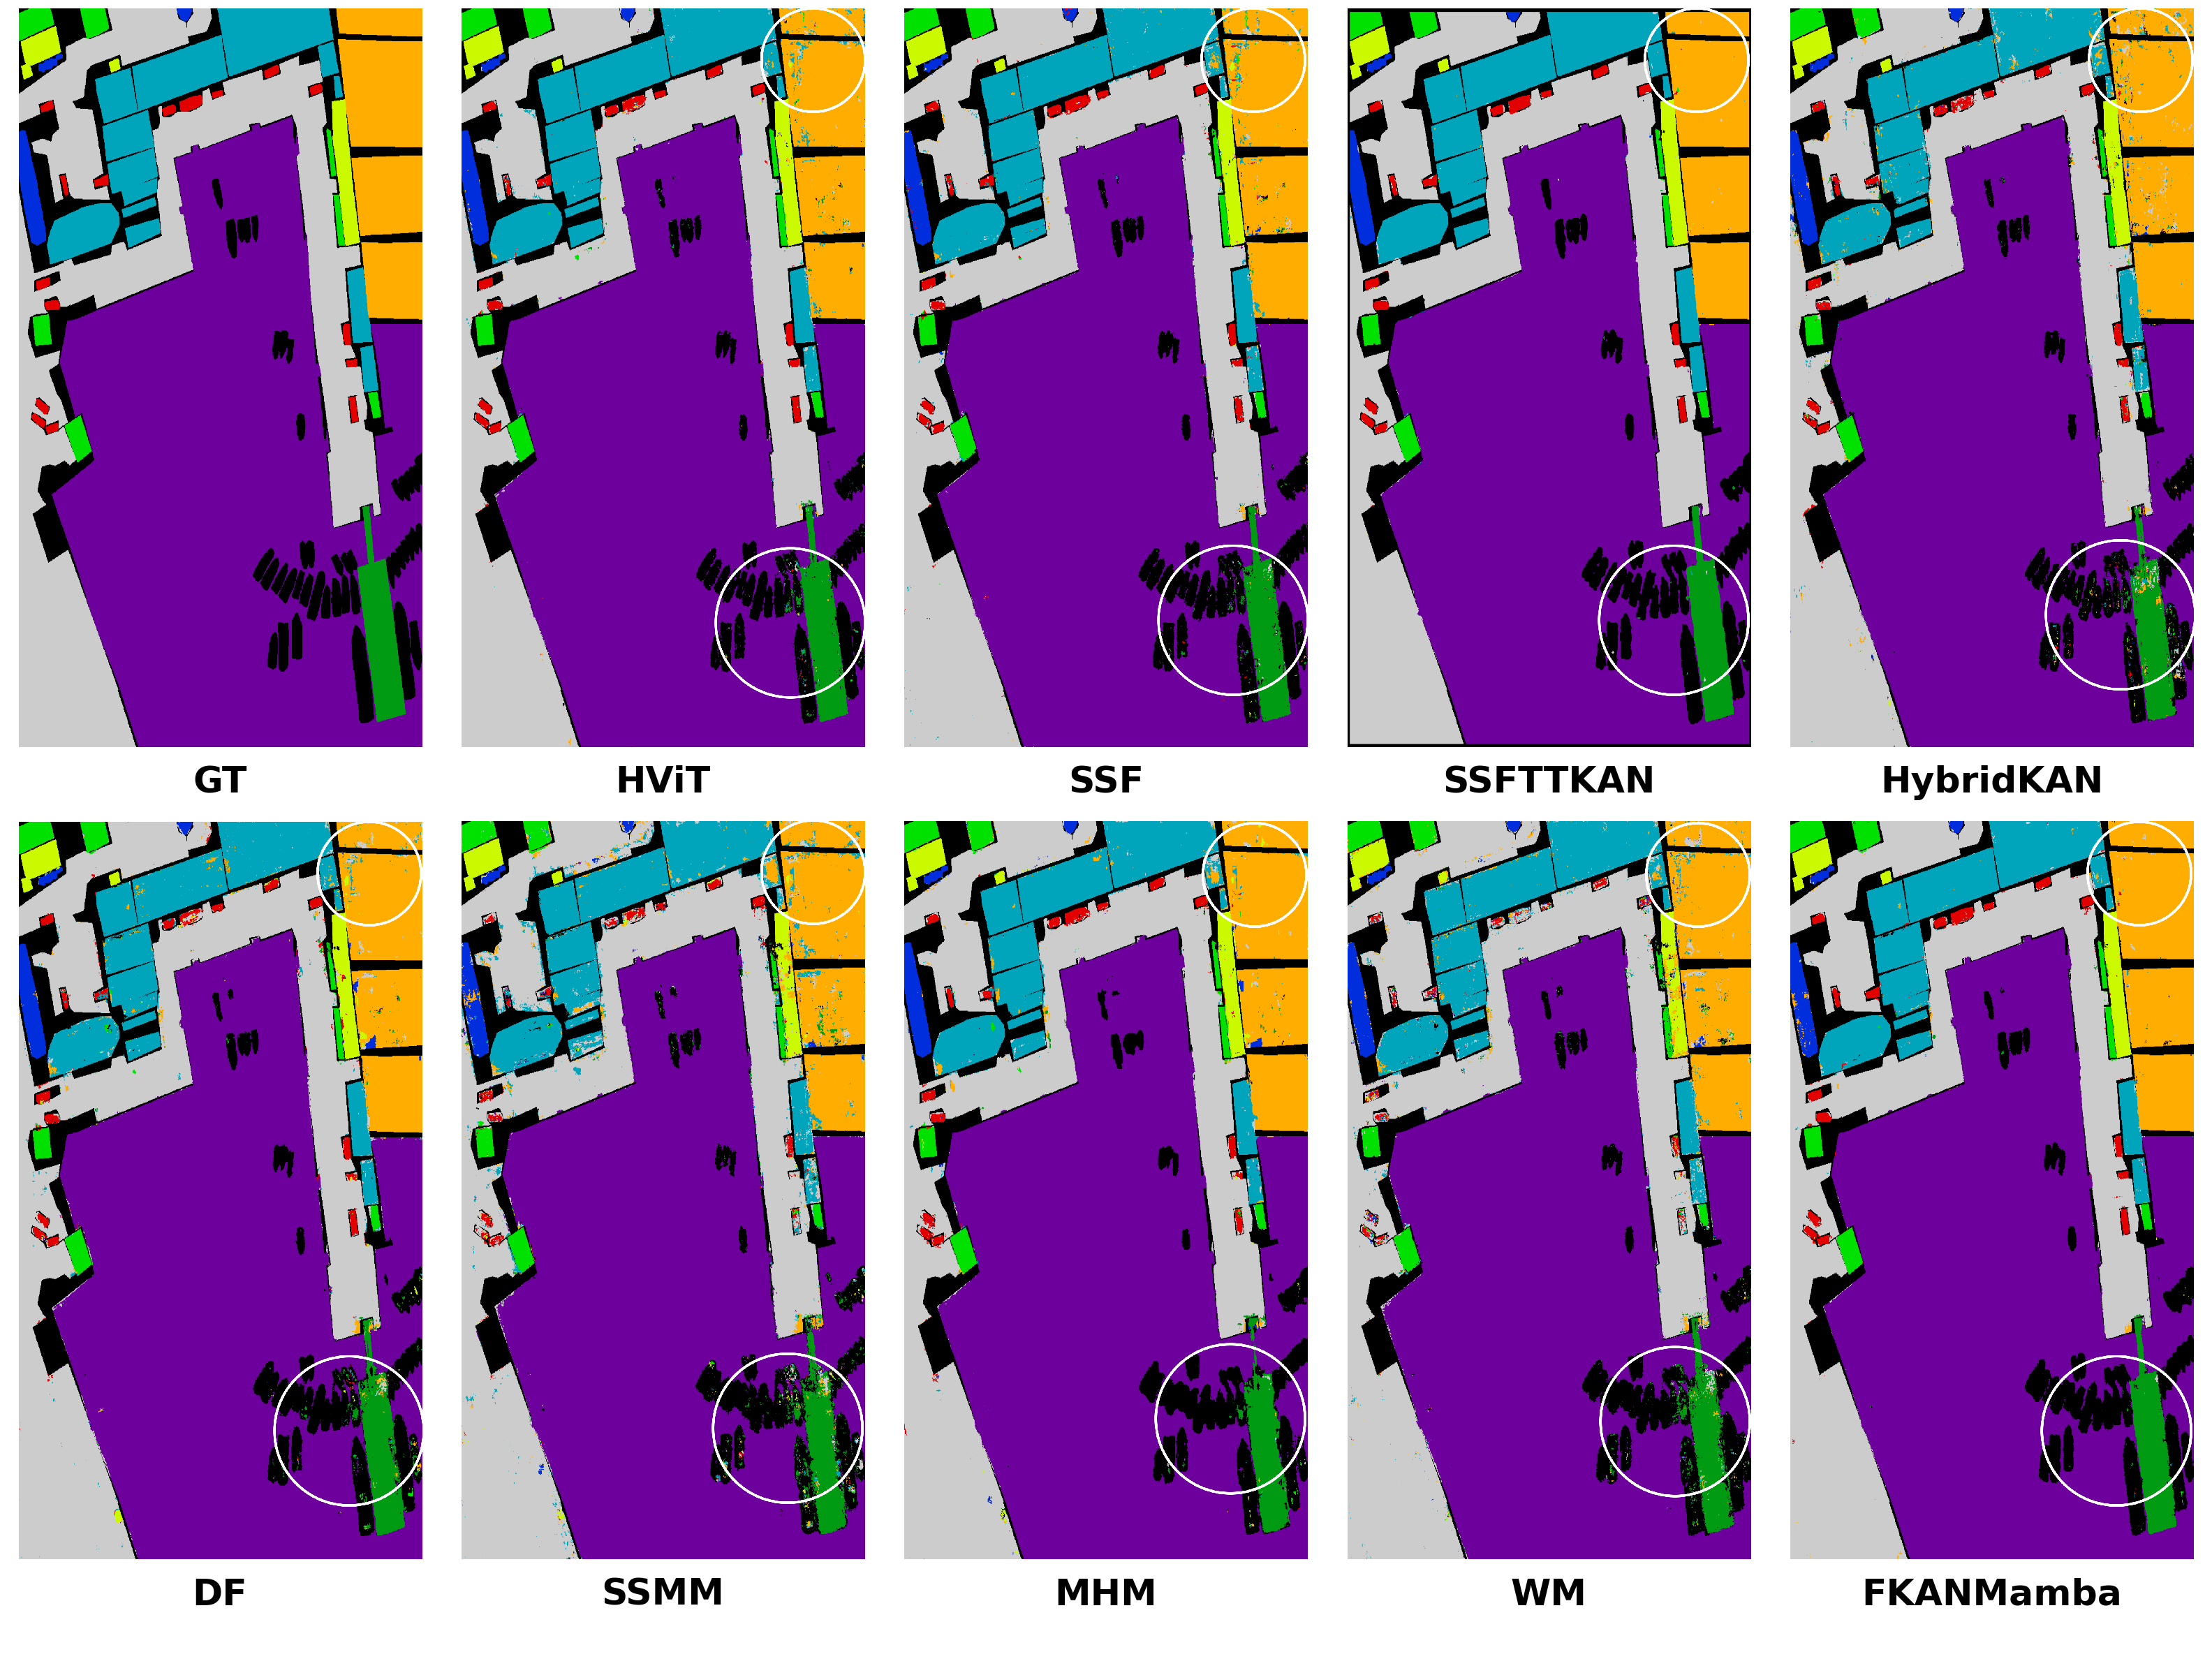
\includegraphics[width=0.98\textwidth]{revision_assets/figures/PI.png}
\caption{Historical within-scene classification maps on PI. External panel labels and layout have been revised for readability; predictions and class colors are unchanged.}
\label{fig:PI}
\end{figure*}

\begin{revision}
Table~\ref{tab:QUH} and Fig.~\ref{fig:QUH} show the historical QUH within-scene results. These scores are single-run observations under overlapping random-pixel sampling and full-scene PCA. They establish neither repeated-run superiority nor spatially independent generalization. Parameter counts measure storage size; the maps are qualitative illustrations rather than independent evidence of deployment performance.
\end{revision}

\begin{table}[!hbt]
    \centering
    \caption{Historical single-run within-scene results. Classwise and overall classification performance (\%) on QUH dataset.}
    
    \resizebox{\columnwidth}{!}{\begin{tabular}{c|cccccccc|c} \hline
        \textbf{Class} &\textbf{HViT}  & \textbf{SSF} & \textbf{SSFTTKAN} & \textbf{HybridKAN} & \textbf{DF} & \textbf{SSMM} & \textbf{MHM} & \textbf{WM} & \textbf{FKANMamba} \\  \hline
        Trees   & \textcolor{red}{\textbf{97.84}} & 96.94 & 97.51 & 97.43  & 96.63 & 95.98 & 96.51 & \textcolor{orange}{\textbf{97.85}} & \textcolor{teal}{\textbf{98.89}} \\ 
        Concrete building   &  \textcolor{red}{\textbf{98.86}} & 97.15 &\textcolor{teal}{\textbf{98.96}} & 96.37 & 98.03 & 95.17 & 96.68 & 97.20 & \textcolor{red}{\textbf{98.86}}\\ 
        Car  & \textcolor{red}{\textbf{84.99}} & 76.76 & \textcolor{teal}{\textbf{91.94}} & 71.74 & 83.06 & 47.31 & 64.11 & 57.58 & \textcolor{orange}{\textbf{87.59}} \\ 
        Ironhide building  & 99.39 & \textcolor{red}{\textbf{ 99.54}} & 99.47 & 99.14& \textcolor{teal}{\textbf{99.87}} & 97.59 & 97.25 & 99.05 & \textcolor{orange}{\textbf{99.82}} \\ 
        Plastic playground  & \textcolor{red}{\textbf{98.60}} &  \textcolor{orange}{\textbf{98.61}} & 96.87 & 97.45 & 97.76 & 95.76 & 97.44 & 95.78 & \textcolor{teal}{\textbf{98.72}} \\ 
        Asphalt road  & \textcolor{teal}{\textbf{97.95}} &  \textcolor{red}{\textbf{97.49}} & 94.60 & 96.37  & 94.91 & 93.30 & 94.87 & 94.46 & \textcolor{orange}{\textbf{97.71 }} \\\hline
        
        \textbf{OA (\%)} & \textcolor{orange}{\textbf{98.07}} & \textcolor{red}{\textbf{ 97.24}} & 96.79 & 96.60 & 96.53 & 94.37 & 95.86 & 95.78 & \textcolor{teal}{\textbf{98.37}} \\ 
        \textbf{AA (\%)} & \textcolor{red}{\textbf{96.27}} & 94.42 &  \textcolor{orange}{\textbf{96.56}} & 93.08  & 95.04 & 87.52 & 91.15 & 90.32 & \textcolor{teal}{\textbf{96.93}} \\ 
        \textbf{$\kappa$} & \textcolor{orange}{\textbf{97.44}}&  \textcolor{red}{\textbf{96.35}} & 95.79 & 95.49 & 95.41 & 92.54 & 94.51 & 94.40 & \textcolor{teal}{\textbf{97.85}} \\ \hline
        
        \textbf{Param} & \num{911046} &\num{2818438} & \num{15061963} & \num{194923} & \num{224166} & \num{22988} & \num{21670} & \num{24646} & \num{36890} \\ \hline
        % \textbf{Time (s)}  & \num{2084} & \num{2049} & \num{2242} & \num{5093} & \num{8582} & \num{24973} & \num{11386} \\ \hline
    \end{tabular}}
    \label{tab:QUH}
\end{table}

\begin{figure*}[t]
\centering
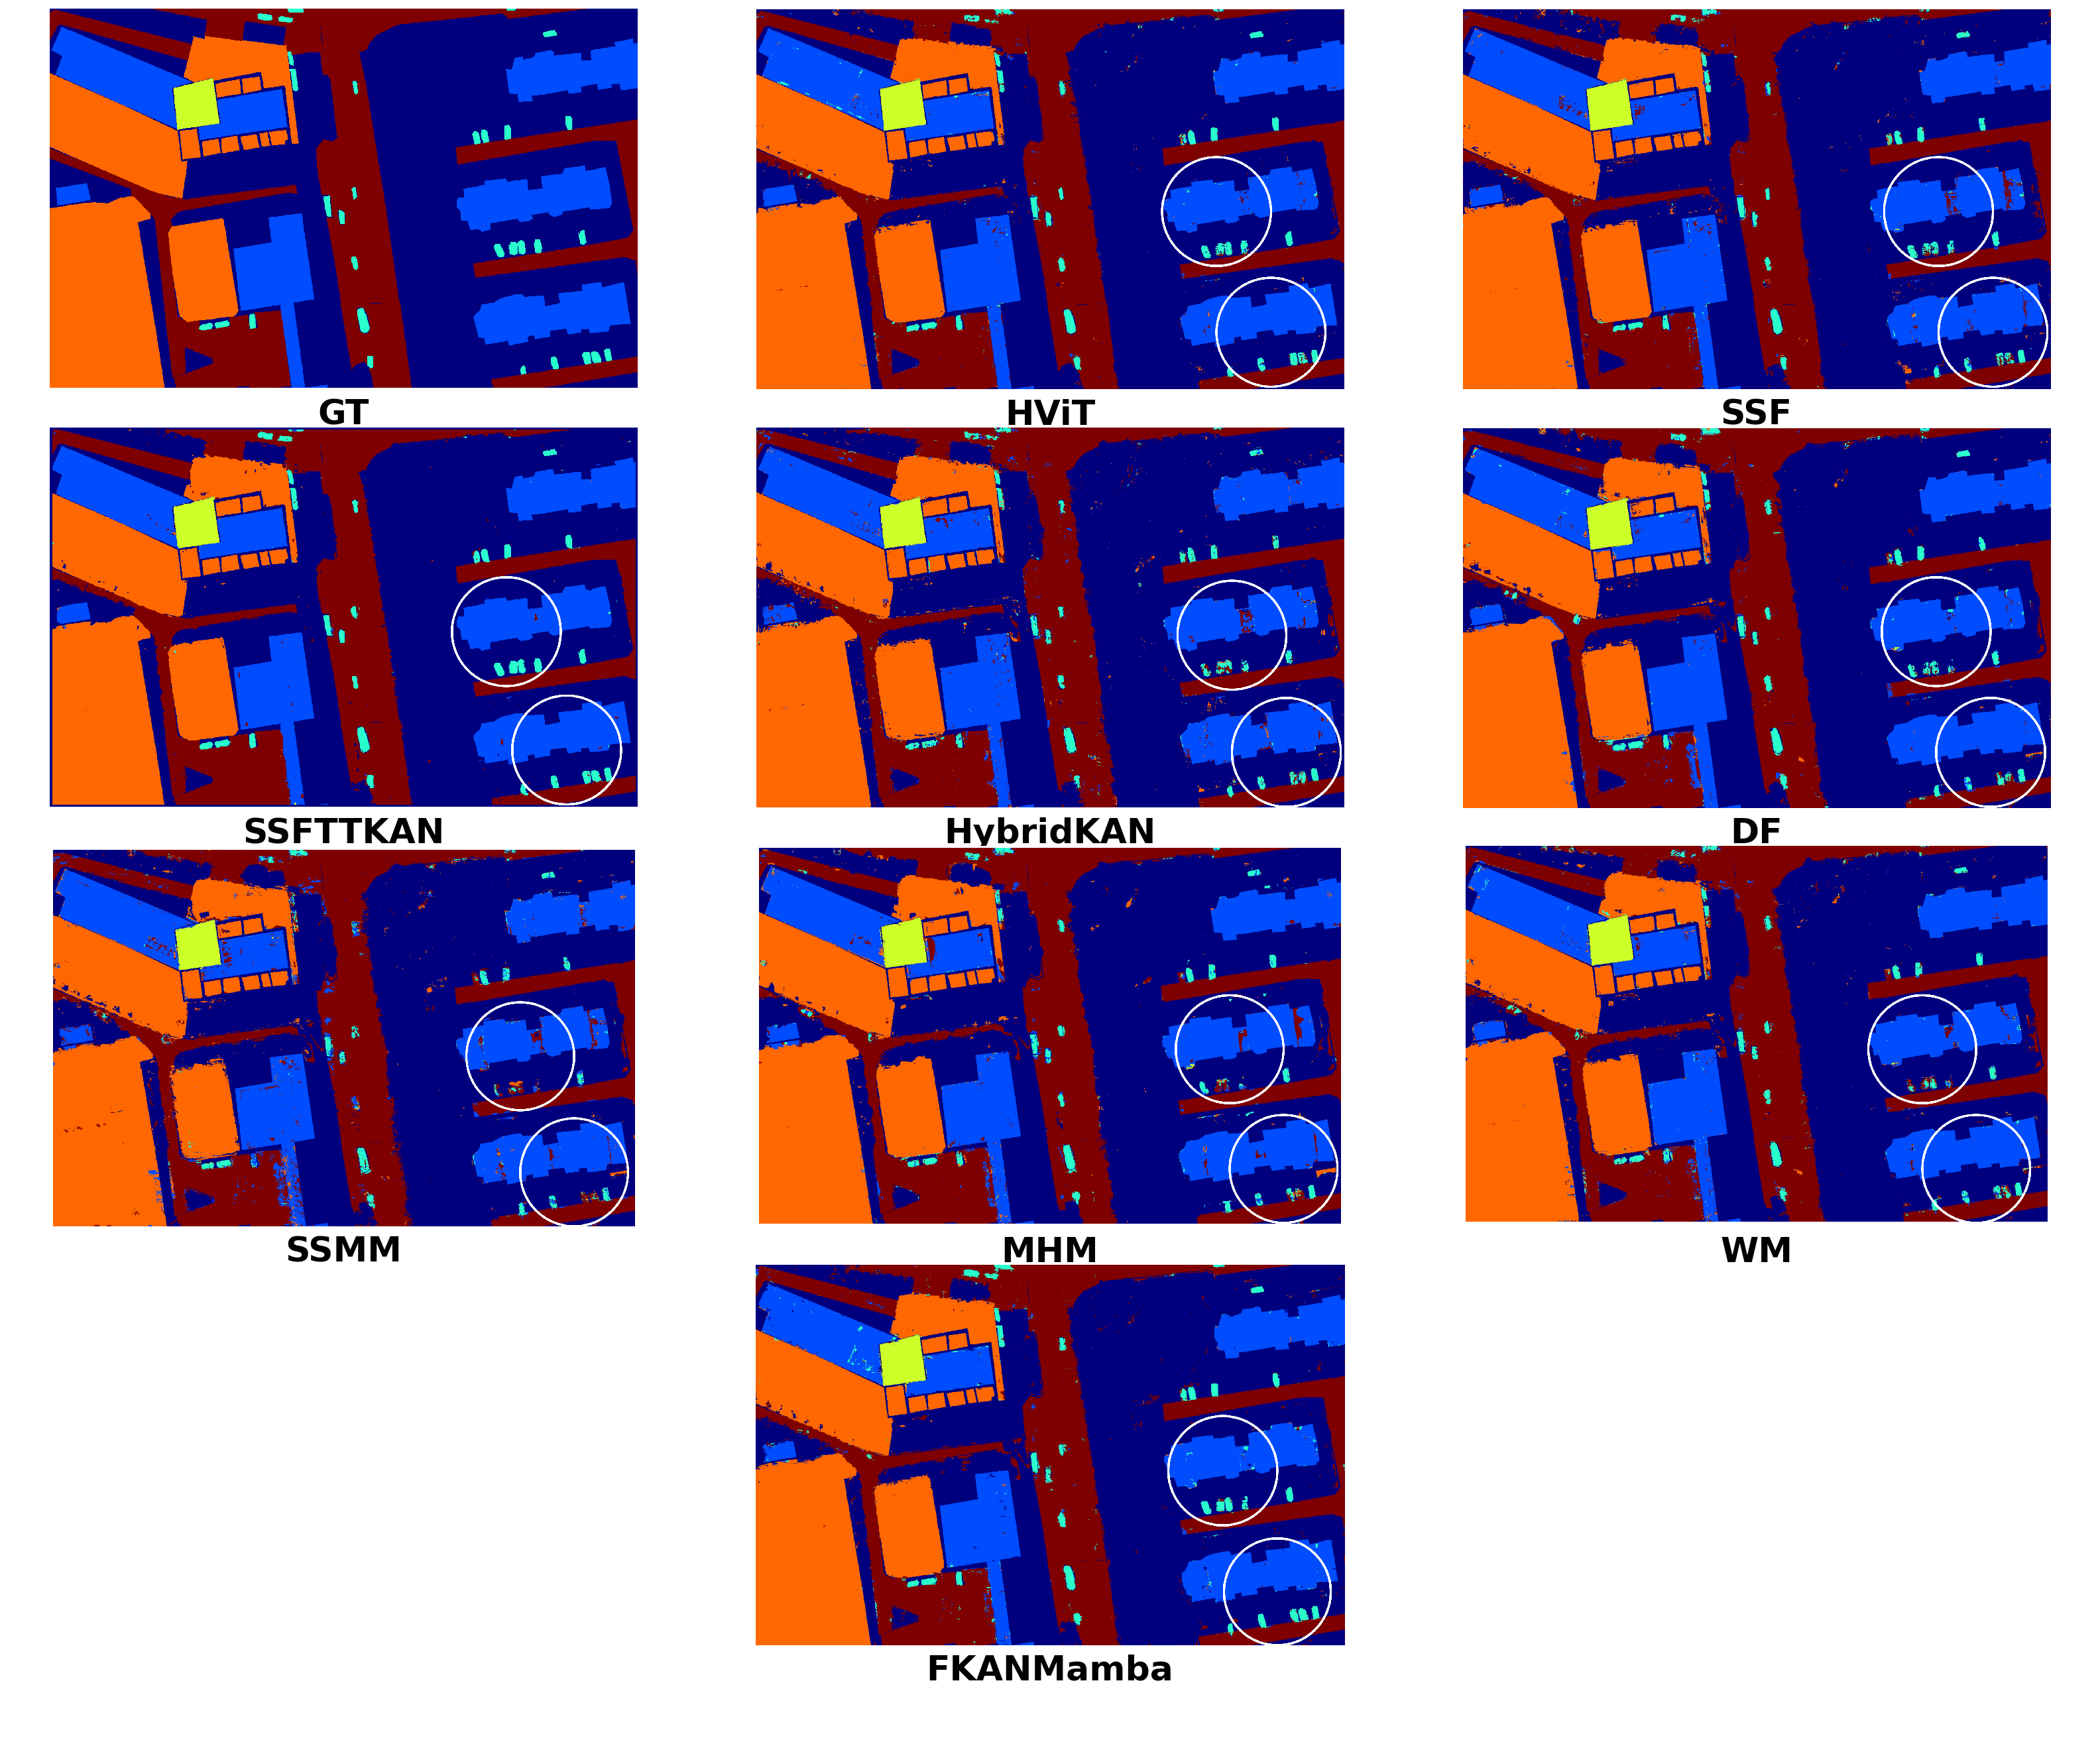
\includegraphics[width=0.98\textwidth]{revision_assets/figures/QUH.png}
\caption{Historical within-scene classification maps on QUH. External panel labels and layout have been revised for readability; predictions and class colors are unchanged.}
\label{fig:QUH}
\end{figure*}

\section{Ablation Study}
\label{sec:ablation}

To examine the contribution of the main design choices in FKANMamba, several ablation experiments are conducted. First, different attention formulations are compared across the five datasets to assess the role of the proposed FastKAN-based attention design. Second, FEB and FSSA are removed separately to evaluate their individual effects. Third, the influence of patch size is analyzed. Finally, different training sample ratios are evaluated to study the accuracy-efficiency trade-off under limited labeled supervision. These experiments provide further insight into how each architectural component affects the final classification performance.

\subsection{FSSA vs. Other Attention Mechanisms}

\begin{revision}
Table~\ref{tab:attention_comparison} contains historical single-run comparisons. Its NA row cannot be assumed identical to the without-FSSA row in Table~\ref{tab:feb_fssa}; their configurations must be recovered before a causal comparison is defensible. The observed attention differences alone do not isolate nonlinear projection capacity, normalization, parameter count, or optimization. New controlled variants are specified in Section~\ref{sec:revision_protocol}.
\end{revision}
\begin{table*}[h]
\caption{Historical single-run within-scene results. Comparison of attention mechanisms on HSI datasets.}
\centering
\begin{adjustbox}{max width=\linewidth}
\begin{tabular}{|l|ccc|ccc|ccc|ccc|ccc|}
\hline
\multirow{2}{*}{\textbf{Dataset}}
& \multicolumn{3}{c|}{\textbf{NA}}
& \multicolumn{3}{c|}{\textbf{MHSA}}
& \multicolumn{3}{c|}{\textbf{CA}}
& \multicolumn{3}{c|}{\textbf{DMHSA}}
& \multicolumn{3}{c|}{\textbf{FSSA}} \\ \cline{2-16}

& OA & AA & $\kappa$
& OA & AA & $\kappa$
& OA & AA & $\kappa$
& OA & AA & $\kappa$
& OA & AA & $\kappa$ \\
\hline

HC
& 77.53 & 57.99 & 73.43
& 95.25 & 91.74 & 94.44
& 90.00 & 79.99 & 88.28
& 92.35 & 87.00 & 91.06
& \textbf{98.63} & \textbf{97.43} & \textbf{98.40} \\ \hline

HH
& 87.92 & 73.59 & 84.71
& 96.39 & 84.11 & 95.43
& 95.06 & 93.36 & 93.74
& 94.15 & 87.29 & 92.61
& \textbf{98.63} & \textbf{95.50} & \textbf{98.27} \\ \hline

PI
& 93.47 & 82.57 & 90.25
& 97.65 & 93.92 & 96.50
& 95.58 & 87.87 & 93.40
& 97.62 & 93.85 & 96.46
& \textbf{98.84} & \textbf{96.93} & \textbf{98.27} \\ \hline

TH
& 94.23 & 89.36 & 93.43
& 97.70 & 93.67 & 97.38
& 97.21 & 93.86 & 96.83
& 97.62 & 96.15 & 97.30
& \textbf{99.31} & \textbf{98.50} & \textbf{99.21} \\ \hline

QUH
& 91.46 & 83.99 & 88.67
& 95.86 & 91.15 & 94.51
& 94.78 & 89.30 & 93.08
& 96.53 & 95.04 & 95.41
& \textbf{98.37} & \textbf{96.93} & \textbf{97.85} \\ \hline

\end{tabular}
\end{adjustbox}

\label{tab:attention_comparison}
\end{table*}














% \begin{figure}[!ht]
%     \centering
%     \begin{adjustbox}{max width=\textwidth}
%     \begin{tikzpicture}
%         \begin{axis}[
%             width=10cm,
%             height=8cm,
%             ylabel= {\textbf{OA (\%) }},
%             xtick={1,2,3,4,5},
%             xticklabels={NA, MHSA, CA, DMHSA, FSSA},
%             legend style={at={(0.98,0.02)}, anchor=south east, font=\scriptsize,
%             rounded corners=2pt,
%             opacity=0.9}, grid=major,
%             grid style={dashed, gray!30},
%             ]
%             \addplot[color=blue!60, mark=*, thick ] coordinates {(1, 77.53) (2, 95.25) (3, 90.00) (4, 92.35) (5, 98.63)};
%             \addlegendentry{HC}
%             \addplot[color=red!60, mark=*, thick] coordinates {(1, 87.92) (2, 96.39) (3, 95.06) (4, 94.15) (5, 98.63)};
%             \addlegendentry{HH}
%             \addplot[color=magenta!60, mark=*, thick] coordinates {(1, 93.47) (2, 97.65) (3, 95.58) (4, 97.62) (5, 98.84)};
%             \addlegendentry{PI}
%             \addplot[color=cyan!70, mark=*, thick] coordinates {(1, 94.23) (2, 97.70) (3, 97.21) (4, 97.62) (5, 99.31)};
%             \addlegendentry{TH}
%             \addplot[color=brown!70, mark=*] coordinates {(1, 91.46) (2, 95.86) (3, 94.78) (4, 96.53) (5, 98.37)};
%             \addlegendentry{QUH}
%         \end{axis}
%     \end{tikzpicture}
%     \hfill
%     \begin{tikzpicture}
%         \begin{axis}[
%             width=10cm,
%             height=8cm,
%             ylabel={\textbf{Kappa ($\kappa$) }},
%             xtick={1,2,3,4,5},
%             xticklabels={NA, MHSA, CA, DMHSA, FSSA},
%              legend style={at={(0.98,0.02)}, anchor=south east,font=\scriptsize,
%             rounded corners=2pt,
%             opacity=0.9},
%             grid=major,
%             grid style={dashed, gray!30},
%             ]
%             \addplot[color=blue!60, mark=*, thick] coordinates {(1, 73.43) (2, 94.44) (3, 88.28) (4, 91.06) (5, 98.40)};
%             \addlegendentry{HC}
%             \addplot[color=red!60, mark=*, thick] coordinates {(1, 84.71) (2, 95.43) (3, 93.74) (4, 92.61) (5, 98.27)};
%             \addlegendentry{HH}
%             \addplot[color=magenta!60, mark=*, thick] coordinates {(1, 90.25) (2, 96.50) (3, 93.40) (4, 96.46) (5, 98.27)};
%             \addlegendentry{PI}
%             \addplot[color=cyan!70, mark=*, thick] coordinates {(1, 93.43) (2, 97.38) (3, 96.83) (4, 97.30) (5, 99.21)};
%             \addlegendentry{TH}
%             \addplot[color=brown!70, mark=*, thick] coordinates {(1, 88.67) (2, 94.51) (3, 93.08) (4, 95.41) (5, 97.85)};
%             \addlegendentry{QUH}
%         \end{axis}
%     \end{tikzpicture}
%     \hfill
%     \begin{tikzpicture}
%         \begin{axis}[
%             width=10cm,
%             height=8cm,
%             ylabel={\textbf{AA (\%)}},
%             xtick={1,2,3,4,5},
%             xticklabels={NA, MHSA, CA, DMHSA, FSSA},
%              legend style={at={(0.98,0.02)}, anchor=south east,font=\scriptsize,
%             rounded corners=2pt,
%             opacity=0.9},
%             grid=major,
%             grid style={dashed, gray!30},
%             ]
%             \addplot[color=blue!60, mark=*, thick] coordinates {(1, 57.99) (2, 91.74) (3, 79.99) (4, 87.00) (5, 97.43)};
%             \addlegendentry{HC}
%             \addplot[color=red!60, mark=*, thick] coordinates {(1, 73.59) (2, 84.11) (3, 93.36) (4, 87.29) (5, 95.50)};
%             \addlegendentry{HH}
%             \addplot[color=magenta!60, mark=*, thick] coordinates {(1, 82.57) (2, 93.92) (3, 87.87) (4, 93.85) (5, 96.93)};
%             \addlegendentry{PI}
%             \addplot[color=cyan!70, mark=*, thick] coordinates {(1, 89.36) (2, 93.67) (3, 93.86) (4, 96.15) (5, 98.50)};
%             \addlegendentry{TH}
%             \addplot[color=brown!70, mark=*, thick] coordinates {(1, 83.99) (2, 91.15) (3, 89.30) (4, 95.04) (5, 96.93)};
%             \addlegendentry{QUH}
%         \end{axis}
%     \end{tikzpicture}
%     \end{adjustbox}
%     \caption{ Comparison of Overall Accuracy (OA), Kappa (\(\kappa\)), and Average Accuracy (AA) for different attention mechanisms on five hyperspectral datasets. NA = no attention; MHSA = multi-head self-attention; CA = cross-attention; DMHSA = differential MHSA; FSSA = FastKAN Spectral–Spatial Attention. FSSA delivers the highest performance across all metrics.}
%     \label{fig:diff_attn}
% \end{figure}


	
		





		





\subsection{Analysis of FEB and FSSA Modules}

\begin{revision}
The historical module table shows dataset- and metric-dependent effects. On QUH, without FEB has OA 98.46\% versus 98.37\% and $\kappa$ 97.96\% versus 97.85\%, while AA falls from 96.93\% to 96.56\%. OA weights classes by frequency whereas AA averages class accuracies equally, so changes need not have the same direction. These small single-run differences do not establish a reliable FEB benefit or harm. No physical mechanism is inferred without supporting analysis. Larger drops after FSSA removal indicate an association for that full variant, not proof that RBF projections alone cause the difference. The new study pairs repetitions and reports per-class outcomes.
\end{revision}
\begin{table*}[h]
\caption{Historical single-run within-scene results. Analysis of the Contribution of Individual Modules in FKANMamba.}
\centering
\begin{adjustbox}{max width=\linewidth}
\begin{tabular}{|c|ccc|ccc|ccc|ccc|ccc|}
\hline
\multirow{2}{*}{\textbf{Model Variant}}
& \multicolumn{3}{c|}{\textbf{HC}} & \multicolumn{3}{c|}{\textbf{HH}} & \multicolumn{3}{c|}{\textbf{PI}} & \multicolumn{3}{c|}{\textbf{TH}} & \multicolumn{3}{c|}{\textbf{QUH}} \\
\cline{2-16} 
& OA & AA & $\kappa$ & OA & AA & $\kappa$ & OA & AA & $\kappa$ & OA & AA & $\kappa$ & OA & AA & $\kappa$ \\
\hline
Without FEB
& 97.53 & 92.97 & 97.11 & 96.23 & 91.91 & 95.24 & 98.47 & 95.15 & 97.71 & 98.80 & 94.33 & 98.64 & 98.46 & 96.56 & 97.96 \\
\hline

Without FSSA
& 85.79 & 73.44 & 83.33 & 89.34 & 76.32 & 86.53 & 92.91 & 81.78 & 89.36 & 93.61 & 90.00 & 92.74 & 91.39 & 84.52 & 88.60 \\
\hline

\textbf{FKANMamba}
& 98.63 & 97.43 & 98.40 & 98.63 & 95.50 & 98.27 & 98.84 & 96.93 & 98.27 & 99.31 & 98.50 & 99.21 & 98.37 & 96.93 & 97.85 \\
\hline
\end{tabular}
\end{adjustbox}
\label{tab:feb_fssa}
\end{table*}



\begin{table*}[!ht]
\caption{Historical single-run within-scene results. Performance comparison for different patch sizes using OA, AA, and $\kappa$ (\%).}
% \caption{Impact of patch size on classification performance in terms of OA, AA, and $\kappa$ (\%).}
\centering
\begin{adjustbox}{max width=\linewidth}
\begin{tabular}{|l|ccc|ccc|ccc|ccc|ccc|}
\hline
\multirow{2}{*}{\textbf{Patch}}
& \multicolumn{3}{c|}{\textbf{HC}} & \multicolumn{3}{c|}{\textbf{HH}} & \multicolumn{3}{c|}{\textbf{PI}} & \multicolumn{3}{c|}{\textbf{TH}} & \multicolumn{3}{c|}{\textbf{QUH}} \\ \cline{2-16}

& OA & AA & $\kappa$ & OA & AA & $\kappa$ & OA & AA & $\kappa$ & OA & AA & $\kappa$ & OA & AA & $\kappa$ \\
\hline

\(2 \times 2\) & 86.79 & 73.21 & 84.52 & 85.64 & 70.05 & 81.85 & 95.46 & 88.28 & 93.23 & 94.29 & 90.66 & 93.49 & 93.44 & 85.02 & 91.30 \\ \hline

\(4 \times 4\) & 92.92 & 86.01 & 91.72 & 93.18 & 84.11 & 91.37 & 96.69 & 88.67 & 95.05 & 96.33 & 92.78 & 95.83 & 95.12 & 89.35 & 93.53 \\ \hline

\(6 \times 6\) & 95.58 & 92.80 & 94.82 & 96.41 & 93.36 & 95.47 & 97.87 & 93.98 & 96.83 & 98.05 & 96.95 & 97.79 & 96.40 & 92.95 & 95.23 \\ \hline

\(8 \times 8\) & 96.94 & 94.35 & 96.42 & 97.42 & 94.25 & 96.74 & 98.27 & 96.61 & 97.42 & 98.56 & 97.39 & 98.36 & 97.15 & 95.40 & 96.22 \\ \hline

\(10 \times 10\) & 98.20 & 96.03 & 97.89 & 98.32 & 96.69 & 97.88 & 98.71 & \textbf{97.10} & 98.08 & 99.14 & 98.38 & 99.02 & 98.28 & 96.66 & 97.73 \\ \hline

\(12 \times 12\) & 98.63 & 97.43 & 98.40 & 98.63 & 95.50 & 98.27 & \textbf{98.84} & 96.93 & \textbf{98.27} & 99.31 & 98.50 & 99.21 & 98.37 & \textbf{96.93} &97.85 \\ \hline

\(14 \times 14\) & \textbf{99.22} & \textbf{98.58} & \textbf{99.09} & \textbf{98.77} & \textbf{97.19} & \textbf{98.45} & 98.77 & 96.57 & 98.17 & \textbf{99.46} & \textbf{98.73} & \textbf{99.38} & \textbf{98.69} & 96.59 & \textbf{98.27} \\ \hline

\end{tabular}
\end{adjustbox}
\label{tab:patch_acc}
\end{table*}










% \begin{table*}[!ht]
% \centering
% \begin{adjustbox}{max width=\linewidth}
% \begin{tabular}{|l||ccc||ccc||ccc||ccc||ccc|}
% \hline
% \multirow{2}{*}{\textbf{Patch}}
% & \multicolumn{3}{c||}{\textbf{HC}} & \multicolumn{3}{c||}{\textbf{HH}} & \multicolumn{3}{c||}{\textbf{PI}} & \multicolumn{3}{c||}{\textbf{TH}}  & \multicolumn{3}{c|}{\textbf{QUH}} \\ \cline{2-16}
%             & $\kappa$ & OA & AA      & $\kappa$ & OA & AA    & $\kappa$ & OA & AA   & $\kappa$ & OA & AA &     $\kappa$ & OA & AA \\
% \hline
% \(2 \times 2\) & 84.52 & 86.79 & 73.21  & 81.85 & 85.64 & 70.05 & 93.23 & 95.46 & 88.28  & 93.49 & 94.29 & 90.66  & 91.3 & 93.44 & 85.02 \\ \hline
% \(4 \times 4\) & 91.72 & 92.92 & 86.01  & 91.37 & 93.18 & 84.11 & 95.05 & 96.69 & 88.67  & 95.83 & 96.33 & 92.78  & 93.53 & 95.12 & 89.35 \\ \hline
% \(6 \times 6\) & 94.82 & 95.58 & 92.8   & 95.47 & 96.41 & 93.36 & 96.83 & 97.87 & 93.98  & 97.79 & 98.05 & 96.95  & 95.23 & 96.40 & 92.95 \\ \hline
% \(8 \times 8\) & 96.42 & 96.94 & 94.35  & 96.74 & 97.42 & 94.25 & 97.42 & 98.27 &96.61   & 98.36 & 98.56 & 97.39  & 96.22 & 97.15 & 95.40 \\ \hline
% \(10 \times 10\) & 97.89 & 98.20 & 96.03 & 97.88 & 98.32 & 96.69 & 98.08 & 98.71 & 97.10  & 99.02 & 99.14 & 98.38	& 97.73 & 98.28 & 96.66 \\ \hline
% \(12 \times 12\) & 98.40 & 98.63 & 97.43 & 98.27 & 98.63 & 95.50  & \textbf{98.27} &\textbf{98.84} &\textbf{96.93} & 99.21 & 99.31 & 98.50 & 97.85 &98.37 & 96.93 \\ \hline
% \(14 \times 14\) &\textbf{99.09} & \textbf{99.22} & \textbf{98.58} & \textbf{98.45} & \textbf{98.77} & \textbf{97.19}  & 98.17 & 98.77 & 96.57 & \textbf{99.38} & \textbf{99.46} & \textbf{98.73} & \textbf{98.27} &\textbf{98.69} & \textbf{96.59} \\ \hline
% \end{tabular}
% \end{adjustbox}
% \caption{\label{tab:patch_acc} Impact of patch sizes on classification performance.}
% \end{table*}



\begin{figure*}[h]
    \centering
    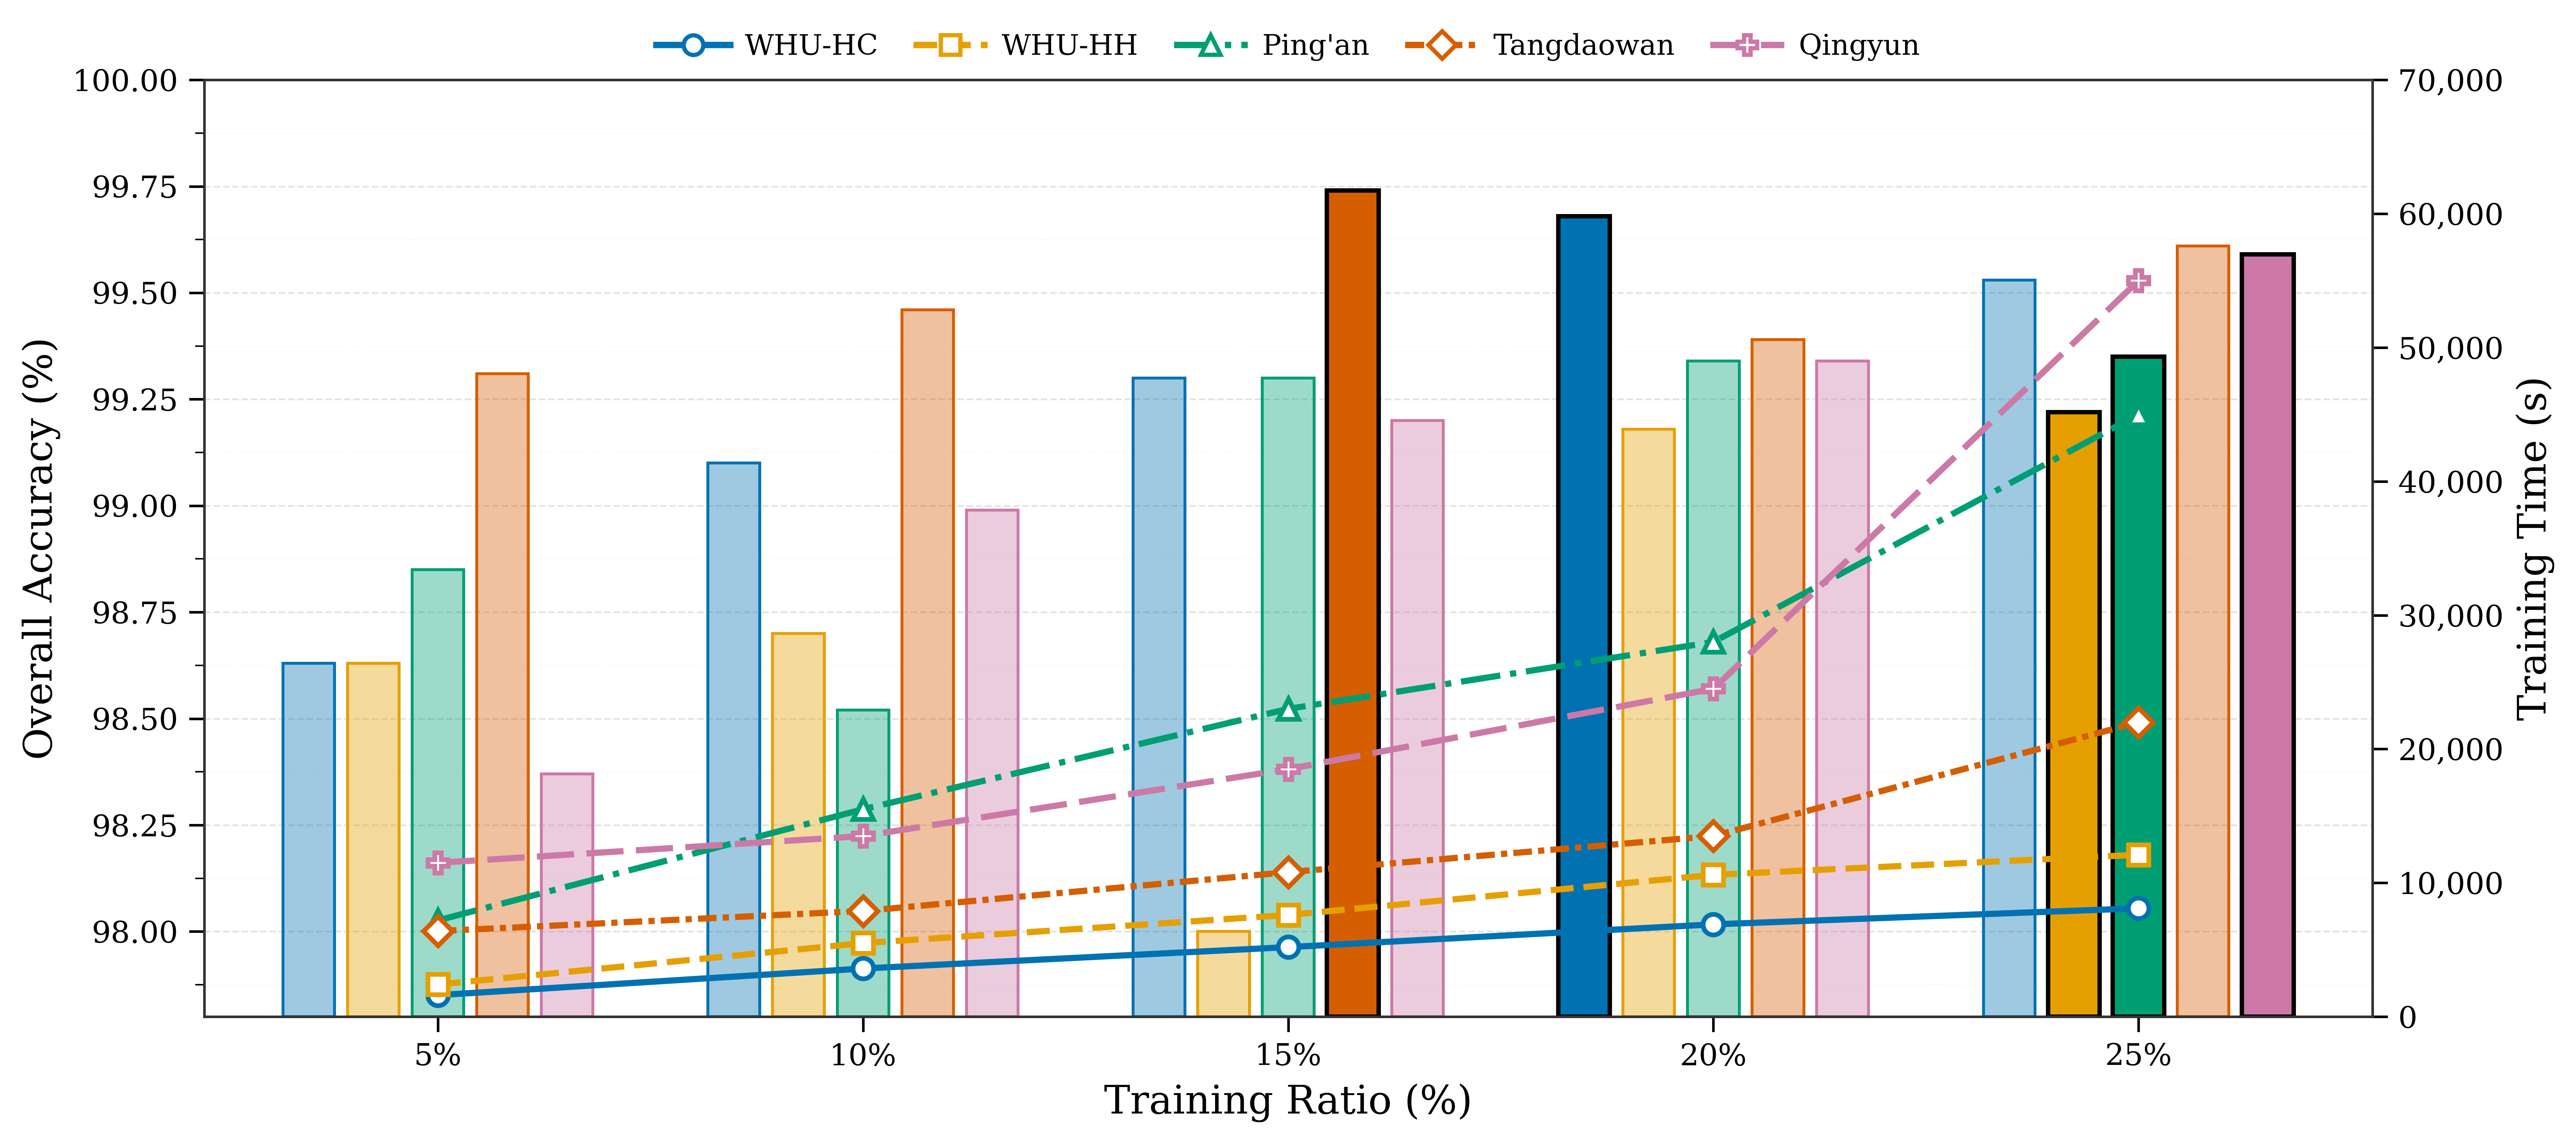
\includegraphics[width=0.80\textwidth]{revision_assets/figures/training_ratio.png}
    \caption{  Training ratio--accuracy--efficiency trade-off of FKANMamba on five HSI benchmarks}
    \label{fig:diff_ratio}
\end{figure*}
\subsection{Impact of Patch Size}
\begin{revision}
Table~\ref{tab:patch_acc} is a historical sensitivity analysis under overlapping patch sampling. Increasing patch size changes both available context and train/test neighborhood overlap, so its accuracy trend cannot be attributed solely to richer context. The new protocol fixes $p=12$ in advance and does not select a patch size using held-out test scores.
\end{revision}
\subsection{Training-Ratio Trade-Off: Accuracy Versus Efficiency}

\begin{revision}
Fig.~\ref{fig:diff_ratio} reports historical accuracy and training cost as the labeled ratio changes within FKANMamba. It is not an inter-model runtime benchmark. The revision fixes the labeled ratio in advance rather than selecting it from held-out test accuracy. The figure does not demonstrate computational superiority over other methods.
\end{revision}

\subsection{Revision Study Protocol and Evidence Status}
\label{sec:revision_protocol}
\begin{revision}
\textbf{Status.} This subsection specifies the revision study; it does not report completed new results. The predeclared matrix has 460 runs: nine methods on five scenes under random sampling, nine methods on HC/HH under spatial sampling, seven controlled variants on HC/HH under both protocols, and a QUH without-FEB check, each with five repetitions. HC/HH are chosen before inspecting new scores because of their fine-grained agricultural categories. All completed scheduled runs, including unfavorable results, will be reported.

\textbf{Sampling and preprocessing.} Repetition $r=0,\ldots,4$ uses split seed $345+r$ and training seed $r$. All methods share the center indices for a dataset, protocol, and repetition. Random sampling is class-stratified 5\%/5\%/90\%. The spatial protocol uses $64\times64$ blocks on HC and $24\times24$ blocks on HH. Label-only feasibility checks found that HH could not satisfy the class-coverage and sample-count constraints at block widths 64, 48, or 32; width 24 was fixed before model training or inspection of accuracy. Blocks are assigned using ground-truth class coverage and count constraints, never spectra or accuracy. Approximately 20\% of eligible blocks are allocated to each of training and validation, with the remainder for testing. Training and validation centers are sampled to target 5\% of each scene's labeled class population where feasible. A center is retained only if its entire $12\times12$ patch fits in its own block. Realized fractions, class counts, excluded pixels, and block masks will be reported; the two scenes' block scales and retained test coverage differ. Infeasible class coverage stops the protocol; classes are not silently removed. Train/validation/test patch-support intersections must be zero. PCA with whitening is fitted only to training-center spectra, then applied unchanged to the scene; no additional spectral standardization is introduced. Full-scene preprocessing is confined to the explicitly labeled historical results.

\textbf{Training and reproducibility.} The FKANMamba schedule remains 50 epochs, batch size 56, and the optimizer settings stated above. The final epoch is evaluated; validation is monitored and test scores are not used for configuration selection. Published baseline settings and any justified deviations require an authenticated implementation record. Each run stores source hashes, exact center indices, block assignments, PCA state, seeds, environment, configuration, training history, checkpoint, predictions, and per-class confusion counts. Five repetitions vary both partitioning and training randomness; they are not five initializations on one fixed split. Missing or failed runs are listed and not silently omitted from summaries.

\textbf{Controlled variants.} The seven variants replace FastKAN Q/K/V with normalized linear maps; replace them with normalized GELU MLPs of width 128; replace FEB's FastKAN gates with corresponding MLP gates; bypass FEB; bypass FSSA while keeping FEB/fusion/recurrence; replace recurrence with mean pooling; or replace recurrence with a selective-Mamba block. Interfaces remain fixed and parameter differences are reported. The selective control has model width 64, state width 64, convolution width 4, expansion 2, and a final-position readout. The TensorFlow selective-scan reference is sequential and is not an optimized CUDA implementation; external reference parity is required before attributing results to a verified conventional Mamba block. These controls address projection capacity and aggregation choices separately, not a newly invented component family.

\textbf{Statistics.} OA, AA, $\kappa$, and per-class accuracy will be reported as mean and sample standard deviation over all five repetitions, together with paired OA differences. Primary OA comparisons use two-sided exact paired sign-flip tests with Holm correction within the random and spatial comparison families. With five pairs the minimum attainable two-sided p-value is 0.0625; lack of significance is not equivalence. These repetitions are conditional on the five scenes and do not establish population-wide or cross-scene generalization.

\textbf{Computational measurements.} Record GPU model, driver, CUDA/cuDNN, framework, CPU, host RAM, precision, batch size, and compilation settings. On an otherwise idle GPU, use FP32, warm-up, synchronized repetitions, batch-1 latency, and batch-56 throughput. Report peak training/inference device memory, first-epoch/steady-state epoch time, and total training time, separating preprocessing and initialization. FLOPs accounting includes both attention calls, RBF projections, and repeated scan operations; state the operation convention and unsupported profiler operations. No comparative efficiency claim is made from partial FLOPs alone. Training-only pilots estimate the budget before test evaluation.

\pending{Insert the five-seed main results, HC/HH spatial results, controlled ablations, QUH FEB analysis, paired statistics, and controlled computational table. The exact public archive URL and final PDF page references remain to be supplied.}
\end{revision}

\section{Conclusion}
\label{sec:conclusion}

\begin{revision}
FKANMamba combines established RBF mappings, two-view attention, and a non-selective affine recurrent readout. The corrected description preserves the implemented operations while separating them from selective Mamba. Historical single-run within-scene results suggest a useful compact classifier, but they do not establish repeated-run superiority, spatially independent generalization, or comparative runtime advantage. The controlled experiments in Section~\ref{sec:revision_protocol} are required before drawing stronger conclusions. \pending{Replace this provisional conclusion with claims supported by the completed revision study.}

\textbf{Limitations.}\label{sec:limitations} Historical spatial overlap and transductive preprocessing limit the interpretation of accuracy. The fixed representative token is not the target spectrum, the two views are not pixel-aligned, and the recurrence is non-selective. The planned spatial comparison covers HC and HH only; it cannot establish transfer between scenes or sensors. Five pipeline repetitions measure variability conditional on these datasets and protocols, with limited power for paired tests. Runtime depends on implementation and hardware, especially for a sequential TensorFlow selective-scan reference. Cross-scene transfer and deployment validation remain outside the present evidence.
\end{revision}
\section*{Acknowledgment}
The following are results of a study on the `Convergence and Open Sharing System' project, supported by the Ministry of Education and the National Research Foundation of Korea.

\bibliographystyle{IEEEtran}
\bibliography{revision_assets/support/sample}

\begin{IEEEbiography}[{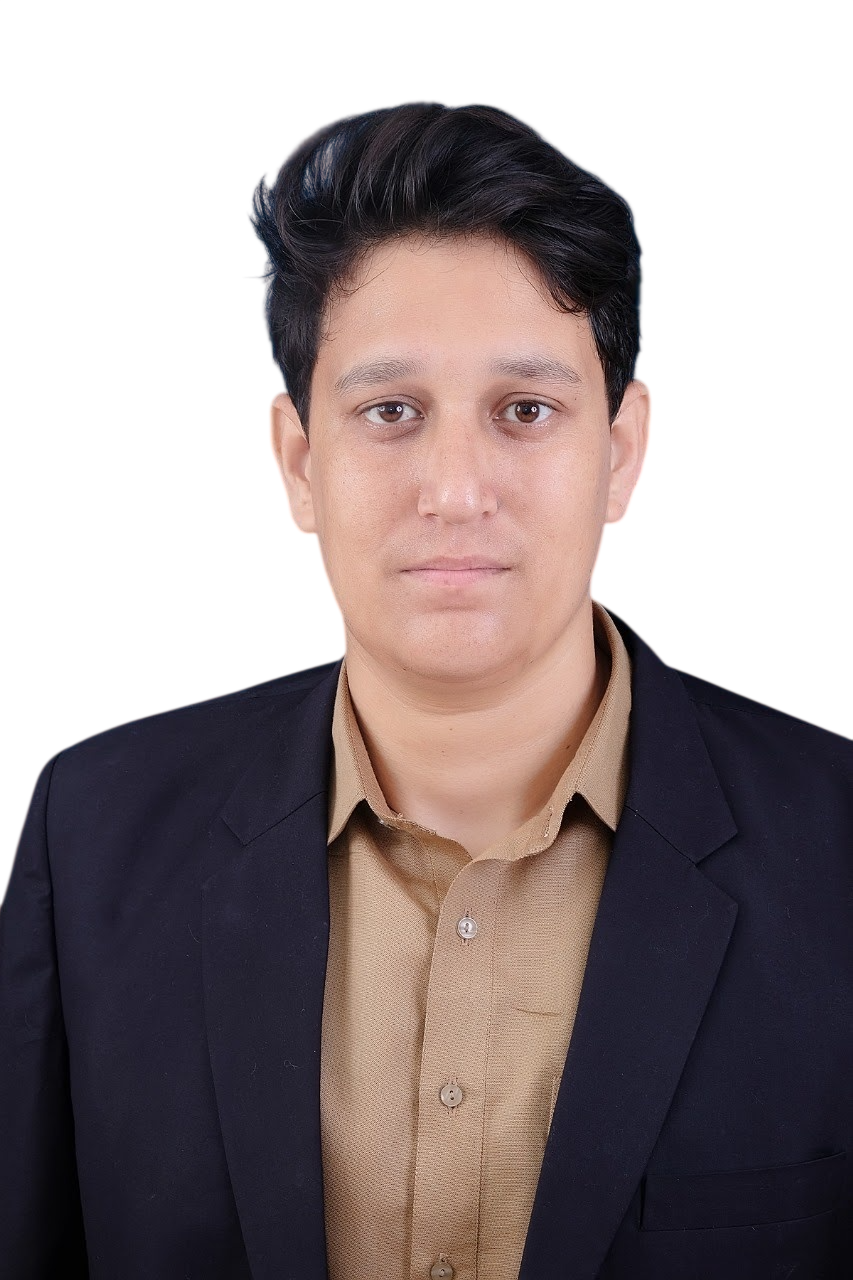
\includegraphics[width=1in,height=1.25in, clip,keepaspectratio]{revision_assets/support/bib/arslan.png}}]{MUHAMMAD ARSLAN} is an Integrated Master's and Ph.D. researcher in the Department of Computer Engineering at Korea Aerospace University, Goyang, Republic of Korea. His research focuses on computer vision and hyperspectral imaging across remote sensing domains. He is actively engaged in remote sensing research, working toward practical and scalable solutions for advanced remote sensing applications.
\end{IEEEbiography}

\begin{IEEEbiography}[{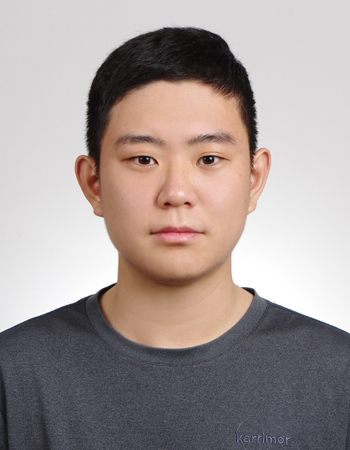
\includegraphics[width=1in,height=1.25in, clip,keepaspectratio]{revision_assets/support/bib/Jaehyeon.jpeg}}]{JAEHYEON KIM} received the M.S. degree in artificial intelligence from Korea Aerospace University, Goyang, Republic of Korea, in 2026. His research interests include trustworthy artificial intelligence, adversarial robustness, and computer vision. He is also interested in vision-language models.
\end{IEEEbiography}

\begin{IEEEbiography}[{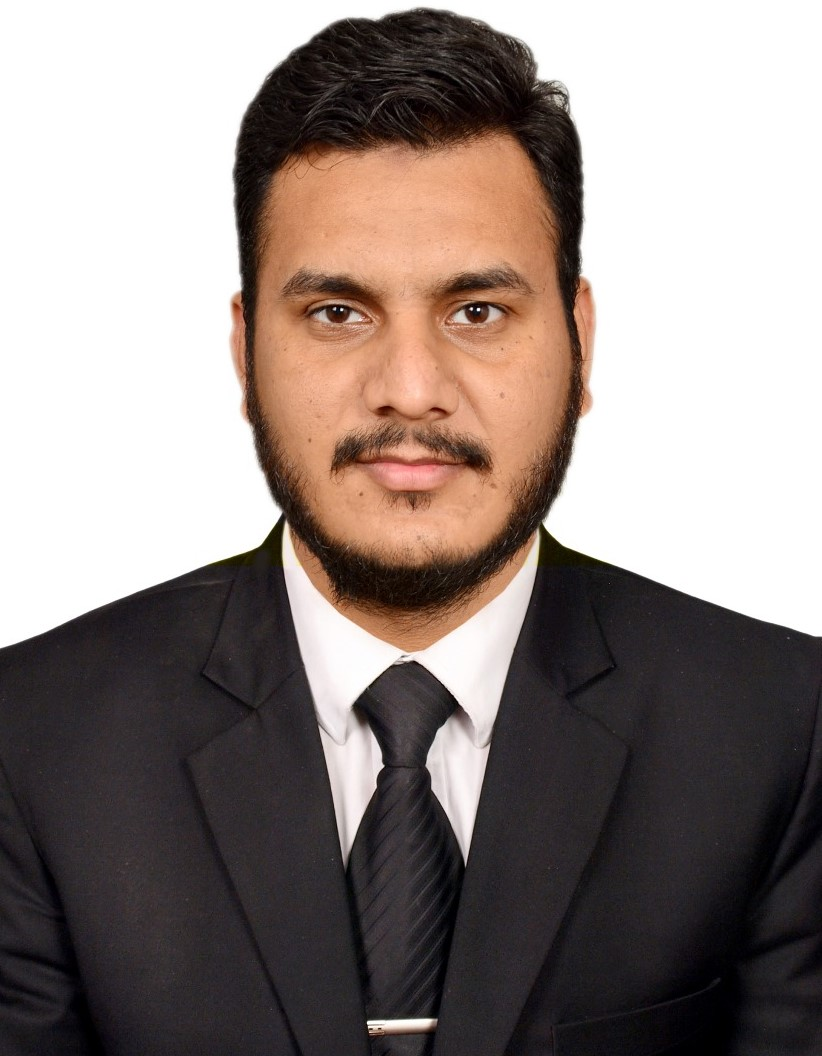
\includegraphics[width=1in,height=1.25in, clip,keepaspectratio]{revision_assets/support/bib/Hassaan.jpg}}]{Muhammad Hassaan Farooq Butt} is a postdoctoral research fellow at the Faculty of Environmental Sciences and Natural Resource Management (MINA), Norwegian University of Life Sciences (NMBU). He earned his Ph.D. in Computer Science and Technology from the University of Electronic Science and Technology (UESTC) in China in 2024, where his research focused on computer vision and hyperspectral imaging across forensic, medical, and remote sensing domains. His doctoral work explored efficient spatial--spectral modeling, leading to the development of several innovative architectures.
\end{IEEEbiography}

\begin{IEEEbiography}[{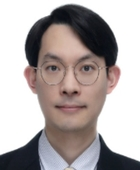
\includegraphics[width=1in,height=1.25in, clip,keepaspectratio]{revision_assets/support/bib/JJ.jpg}}]{JAY HOON JUNG} received the Ph.D. degree in computer science from the State University of New York at Stony Brook. He is currently an Assistant Professor in the Department of Artificial Intelligence at Korea Aerospace University. His primary research delves into uncovering the foundational principles of artificial neural networks. He aspires to leverage these insights to develop quantum algorithms for deep learning. Additionally, he is invested in developing efficient algorithms for remote sensing.
\end{IEEEbiography}

\EOD
\end{document}

